\documentclass[11pt,a4paper,twoside,UTF8]{report}

\usepackage{CJKutf8}

\usepackage{setspace}
% avoid too much space automatically padded between paragraphs to fill a page:
\raggedbottom
\usepackage{graphics}
\usepackage{thesis} 
\usepackage{rotating}

% packages for including image
\usepackage{graphicx}

% set margin
\usepackage[inner=4cm,outer=2.5cm]{geometry}

% packages for math equations 
\usepackage{amsfonts,amsmath,amssymb}
\usepackage{mathptmx,mathtools}
\usepackage{bm}

% packages for table layout
\usepackage{booktabs}
\usepackage{multirow}
\usepackage{threeparttable}

% packages for algorithm layout
\usepackage{algorithm}
\usepackage{algorithmic}

\usepackage[dvips]{epsfig}

% set font style
\usepackage[mono=false]{libertine}

% font size for chapter title
\usepackage{sectsty}
\chapternumberfont{\LARGE}
\chaptertitlefont{\huge}

% package for blank page
\usepackage{afterpage}

% style for links
\usepackage[colorlinks=true,linkcolor=blue,citecolor=blue]{hyperref}

% package for setting header style
\usepackage{fancyhdr}

\usepackage{biblatex}
\addbibresource{database.bib}

\def\bbR{\mathbb{R}}
\def\bbE{\mathbb{E}}
\def\bbX{\mathbb{X}}
\def\bbP{\mathbb{P}}
\def\bbS{\mathbb{S}}
\def\bbI{\mathbb{I}}
\def\bR{\mathbf{R}}
\def\bz{\mathbf{z}}
\def\bfe{\mathbf{e}}
\def\br{\mathbf{r}}
\def\bT{\mathbf{T}}
\def\bfx{\mathbf{x}}
\def\bp{\mathbf{p}}
\def\bq{\mathbf{q}}
\def\ba{\mathbf{a}}
\def\bg{\mathbf{g}}
\def\bv{\mathbf{v}}
\def\bu{\mathbf{u}}
\def\bl{\mathbf{l}}
\def\bX{\mathbf{X}}
\def\bY{\mathbf{Y}}
\def\bW{\mathbf{W}}
\def\bQ{\mathbf{Q}}
\def\bK{\mathbf{K}}
\def\bM{\mathbf{M}}
\def\bN{\mathbf{N}}
\def\bzero{\mathbf{0}}
\def\caN{\mathcal{N}}
\def\caX{\mathcal{X}}
\def\caG{\mathcal{G}}
\def\bOmega{\bm\Omega}
\def\bomega{\bm\omega}
\def\bSigma{\bm\Sigma}
\def\bsigma{\bm\sigma}
\def\bvarsigma{\bm\varsigma}
\def\btheta{\bm\theta}
\def\bdelta{\bm\delta}
\def\bDelta{\bm\Delta}
\def\bPhi{\bm\Phi}
\def\bmV{\bm V}
\def\bxi{\bm\xi}
\def\brho{\bm\rho}
\def\bnu{\bm\nu}
\def\bmeta{\bm\eta}
\def\bvarrho{\bm\varrho}
\def\bvarrho{\bm\varrho}
\def\det{\mathrm{det}}
\def\tr{\mathrm{tr}}
\def\trans{^\mathrm{T}}
\def\diag{\mathrm{diag}}
\def\adj{\mathrm{adj}}
\def\inv{^{-1}}
\def\caJ{\mathcal{J}}
\def\caT{\mathcal{T}}
\def\bfb{\mathbf{b}}
\def\bmb{\bm b}
\def\Exp{\mathrm{Exp}}
\def\Log{\mathrm{Log}}
\def\half{\frac{1}{2}}
\def\SO{\mathrm{SO}}
\def\SE{\mathrm{SE}}
\def\sefr{\mathfrak{se}}
\def\sofr{\mathfrak{so}}

\def\argmin{\operatorname*{arg\,min}}
\def\argmax{\operatorname*{arg\,max}}

\newcommand{\Norm}[1]{
    \left\| #1 \right\|
}
\newcommand{\norm}[1]{
    \left| #1 \right|
}
\newcommand{\deriv}[2]{
	\frac{\mathrm{d}\, #1}{\mathrm{d}\, #2}
}
\newcommand{\pderiv}[2]{
  \frac{\partial\, #1}{\partial\, #2}
}
\newcommand{\halfof}[1]{
  \frac{#1}{2}
}
\newcommand{\vIm}[1]{
\left[#1\right]_\Im
}
\newcommand{\indep}{\rotatebox[origin=c]{90}{$\models$}}

\newcommand\given[1][]{\:#1\vert\:}

\newenvironment{Rfont}{\fontfamily{pcr}\selectfont}{\par}


\DeclareTextFontCommand{\textR}{\Rfont}
\DeclareMathOperator{\Var}{\widehat{Var}}




% =======================================================
\begin{document}

% cover page information
\thesistitle{Research on Machine Learning for Drug Discovery and Precision Medicine}
\authorname{ZHAO, Kai}
\degree{Doctor of Philosophy}
\programme{Biomedical Sciences}
\supervisor{Prof. So Hon Cheong}
\submitdate{July 2020}

\committee{
    \begin{tabular}{ r l}
	Professor & CHENG Sze Lok (Chair)\\
	Professor & SO Hon Cheong (Thesis Supervisor)\\
	Professor & CHEN Yangchao (Committee Member)\\
    Professor & SHAM Pak Chung (External Examiner)
    \end{tabular}
}
\coverpage

% 1.5 or 2 line spacing for normal texts, required by GS of CUHK
\setstretch{1.25}

% cover page.
\pagenumbering{roman}

% abstract
\abstractpage

% acknowledgement
\acknowledgementpage

%dedication
\dedicationpage

% preamble sections
\tableofcontents
\listoffigures
\listoftables
\chapter*{Symbols and Acronyms}
\addcontentsline{toc}{chapter}{Symbols and Acronyms}

In general, we denote a scalar by an italic lower case letter,
a vector by a roman lower case bold letter,
and a matrix by a roman upper case bold letter respectively, e.g., 
$a \in \bbR $, $\mathbf{v} \in \bbR^n$ and $\mathbf{M} \in \bbR^{p \times q}$, with any exceptions to be mentioned in the context case by case.

An identity matrix is written as $\mathbf{I}$. Specifically, an $n\times n$ identity matrix is written as $\mathbf{I}_n$.
A zero matrix or vector is written as ${\bf 0}$. Specifically, an $m\times n$ zero matrix is written as ${\bf 0}_{m\times n}$.

Specialized symbols and major acronyms are defined as follows:

\newpage

\noindent
$p(\cdot)$                     \hfill the probability density function (PDF) \\
$\Pr(\cdot)$                   \hfill the probability value \\
$\mathbb{E}(\cdot)$            \hfill  the expectation \\
$\bm\Sigma$                    \hfill a covariance matrix \\
$\bN(\mu,\bSigma)$             \hfill a normal distribution with mean $\mu$ and covariance $\bSigma$ \\
$\epsilon$                     \hfill a noise vector \\
${\bf e}(\cdot)$               \hfill an error/residual function \\
$\mathbf{H}$                   \hfill Hessian matrix \\
$\tr(\cdot)$                   \hfill trace of a matrix \\
$\det(\cdot)$                  \hfill determinant of a matrix \\

\newpage
\noindent
DNN       \hfill deep neuron network                  \\
GBM       \hfill gradient boosting machine            \\
SVM       \hfill support vector machine               \\
CF        \hfill causal forests                       \\
RF        \hfill risk factors                         \\
ML        \hfill machine learning                     \\
EN        \hfill elastic net                          \\
ITE       \hfill individualized treatment effects         \\
TE        \hfill treatment effects                    \\
tx        \hfill treatment                            \\
CM        \hfill cardiometabolic                      \\
GWAS      \hfill genome-wide association studies      \\
CNV       \hfill copy number variation                \\
SML       \hfill supervised machine learning          \\ 
MCMC      \hfill Markov chain Monte Carlo             \\
GRF       \hfill general causal forests               \\
CF        \hfill causal forests                       \\
CV        \hfill cross validation                     \\
MSE       \hfill mean squared error                   \\
CI        \hfill confidence interval                  \\



% initialization
\newpage
\pagenumbering{arabic}
% \pagestyle{headings}
\pagestyle{fancy}
\renewcommand{\headrulewidth}{1pt}
\fancyhf[lh,rh,ch]{}
\fancyhf[leh]{\leftmark}
\fancyhf[roh]{\rightmark}

% 1.5 or 2 line spacing for normal texts, required by GS of CUHK
\setstretch{1.5}

% =======================================================
% insert the chapters
\chapter{Introduction}
  \section{Drug Discovery Today}
    New drug development is a lengthy and costly process, and a recent study reported an average cost of $\sim$ 2558 million US dollars in developing a new drug \cite{dimasi2016innovation}. Part of the reason of the high cost is due to the high failure rate of preclinical drug candidates, which is largely caused by lack of efficacy of these candidates; this indicates that the wrong target is pursued \cite{shih2018drug}. Computational drug repositioning and target discovery may serve as a new way to shorten the process of drug development, due to the lower cost and more established safety profile of existing drugs \cite{dudley2011exploiting}. A number of in silico approaches have been developed for drug repositioning and target discovery and are reviewed elsewhere \cite{hodos2016silico,vanhaelen2017design,kandoi2015prediction}. With the rapid rise of machine learning (ML) technologies in the past decade, there has been a rising interest in applying ML methods in drug repositioning or target discovery. 

    Machine learning refers to a vast number of methods for computers to "learn" and gain insight into data without human interference. These methods are classified into two categories: supervised and unsupervised. Supervised machine learning methods are models for prediction or estimation based on one or more inputs. They are called supervised methods, as their learning is "supervised" by known output values. On the other hand, unsupervised machine learning methods can be used to detect relationship or patterns underlying "unlabeled" data. Here we focus on supervised learning methods for classification, since in most cases studies related to drug discovery using ML are the application of classification algorithms. One approach to drug repurposing is to employ drug expression profiles as predictors (i.e., features) to predict a drug’s treatment potential. The outcome variable can be the drug category (e.g., whether it is a cardiovascular or anticancer agent) or whether the drug is indicated for a particular disorder (e.g., whether the drug is indicated for diabetes). In the former case, drugs that are classified into categories other than its own indications may be considered for repositioning. In the latter case, drugs with high predicted probabilities but not indicated for the disorder may serve as candidates for repositioning. Additionally, we may also interested in whether the expression profile induced by genetic perturbation (e.g. over-expression or knock down) showed similar pattern to expression profiles of drugs considered as treatments for specific disease, since in this case the perturbed gene can be considered as promising target for the disease. Note that indications for drugs can easily be obtained from publicly available resources such as the Anatomical Therapeutic Chemical (ATC) Classification System \cite{wei2013development}. An important advantage is that ML algorithms are abundant and in rapid development, and any existing or new algorithms can be applied without much modification.

    With the growth of availability of biomedical data, especially “omics”, computational methods can offer a fast, cost-efficient and systematic way to priority promising drug target and drug repurposing candidates for various diseases. The approach has several advantages. Specifically, finding new indications for existing drugs, an approach known as drug repositioning or repurposing, can serve as a useful strategy to shorten the development cycle. Repurposed drugs can be brought to the market in a much shorter time-frame and at lower costs. Meanwhile, computational drug target identification also can speed up the drug development by prioritizing the most promising drug target candidates in a short time, greatly reducing the time in seeking for potential drug targets. 

    There has been increasing interest in computational drug repositioning recently, in view of the rising cost of new drug development. Hodos et al. provided a comprehensive and updated review on drug repositioning \cite{hodos2016silico}, and G. Kandoi et. al. briefly reviewed applications of machine learning and system biology on discovery of target proteins \cite{kandoi2015prediction}. For the purpose of repositioning, similarity-based methods \cite{gottlieb2011predict,oh2014network,liu2015similarity,luo2016drug,napolitano2013drug,li2012new} usually were employed to explore repositioning opportunities, but as noted by Hodos et al., the dependence on data in the “nearby pharmacological space” might limit the ability to find medications with novel mechanisms of actions. Another related methodology is the network-based approach \cite{lotfi2018review}, which typically requires data on the relationship between drugs, genes and diseases as well as connections within each category (e.g. drug-drug similarities). It still constraints by the focus on a nearby pharmacological space and the choice of tuning parameters in network construction or inference is often ad hoc \cite{ferrero2017silico}. The present work is different in that we apply a broad framework for repositioning and we do not focus on one but many different kinds of learning methods. There is comparatively less reliance on known drug mechanisms or the "nearby pharmacological space" as we let the different algorithms "learn" the relationship between drugs, genes and disease in their own ways. We note that kernel-based ML methods such as support vector machine (SVM) are also based on some sort of similarity measures. A related work \cite{napolitano2013drug} have also examined SVM as a promising ML approach for drug repositioning and identified several interesting candidates. However, here our focus is different in that we considered a variety of other approaches and SVM is one of the methods which falls under the broader framework of ML for repositioning. 

    Although computational drug repositioning has attracted increased attention recently, few studies focus on psychiatric disorders, compared to other areas like oncology. Psychiatric disorders are leading causes of disability worldwide \cite{vigo2016estimating}, however there have been limited advances in the development of new pharmacological agents in the last two decades or so \cite{hyman2013psychiatric}. Development of new therapies is also limited by the difficulty of animal models to fully mimic human psychiatric conditions \cite{nestler2010animal}. Investment by drug companies has in general been declining \cite{hyman2013psychiatric} , and new approaches for drug discoveries are very much needed in this field. We will explore repositioning opportunities for schizophrenia along with depression and anxiety disorders. Here depression and anxiety disorders are analyzed together as they are highly clinically comorbid \cite{kessler2015anxious,otowa2016meta}, show significant genetic correlations\cite{otowa2016meta}, and share similar pharmacological treatments \cite{ballenger2000anxiety}.
    
    Meanwhile, we also have witnessed a rise in the interest of computational target discovery in recent years. G. Kandoi et. al. briefly reviewed applications of machine learning and system biology on discovery of target proteins \cite{kandoi2015prediction}. These studies explored different biological properties by machine learning methods to identify druggable targets \cite{bakheet2009properties,fauman2011structure,li2007prediction}. Biological features of human proteins like amino acid composition and amino acid property group composition were studied by a sequence-based prediction method to identify drug target proteins, and a comprehensive comparison of several machine learning methods was conducted \cite{kumari2015identification}. In another study, eight key properties of human drug target were extracted, and learned by support vector machine (SVM) to discover new targets; similar studies extracted simple physicochemical properties from known drug targets and explored the predictive power of these properties \cite{li2007prediction,emig2013drug}. Topological features of human protein–protein interaction network also were utilized by network based methods to identify potential drug targets \cite{li2015large}. In a recent study, gene-disease association data from Open Targets was explored by four different machine learning methods, including deep neuron networks, to find novel targets, and a large proportion of new targets identified were supported by previous literatures \cite{ferrero2017silico}. Dorothea Emig et. al. proposed an integrated network-based method to predict drug targets based on disease gene expression profiles and a high-quality interaction network, and some novel drug targets for scleroderma and other types of cancer were presented \cite{emig2013drug}. A most recent study proposed pairwise learning and joint learning methods constructed on chemically and genetically perturbed gene expression profiles, and outcome variable was defined as highly correlated pair given by the direct correlation calculation \cite{sawada2018predicting}. These studies aim to discover new targets by making use of structural attributes of proteins or properties of known targets, so targets with similar properties usually are identified, but drug targets with novel mechanisms are difficult to identify using this kind of approaches. Network based methods for target discovery, as mentioned previous, rely on known nearby targets to inference potential relationship, so they suffers the same drawback. 

    Even though repositioned drugs can be brought into market in a much shorter time, drug repositioning may not always be feasible (for example due to side-effects of existing drugs), and drug repositioning and target discovery can complement each other in drug development and pharmacological research. Additionally, in traditional drug development majority of drugs fail to complete the development process due to lack of efficacy, indicating that the wrong target is pursued \cite{shih2018drug}.Usually, a drug target is selected via analyzing how its function influences the disease. However, this process is time-consuming, because investigating a large number of potential targets is usually necessary for finding an ideal one \cite{phoebe2008identifying}. Computational methods can be utilized to hasten this process by prioritizing promising drug targets. 

  \section{Precision Medicine}
    Researchers have discovered hundreds of genes that harbor variations contributing to human illness. For example, genome wide association studies have identified 108 schizophrenia-associated genetic loci \cite{schizophrenia2014biological}. Genetic variability leads to patients response differently to dozens of treatments, and molecular causes of some diseases have been targeted in research. Direct-to-consumer (DTC) companies take advantage of DNA tests to provide genetic insights into personal traits and disease risks \cite{ng2009agenda}. The genetic testing can improve disease prevention \cite{heshka2008systematic}. Moreover, scientists have been beginning to utilize genetics or other molecular mechanisms to better predict patients' responses to targeted therapy \cite{hamburg2010path}. Particularly, there are successful examples in translation of cancer genomics into therapeutics and diagnostics. For instance, doctors recommend KRAS mutation testing for patients with colon or lung cancer before the initiation of  EGFR-targeted therapies; moreover, patients with RAS mutations are more likely to  benefit from pharmacological inhibition of the kinases MEK1 and 2 \cite{lievre2008kras}. Another clinically relevant question to individuals is how a risk factor will affect them individually. A more recent example is that the pandemic of coronavirus-19 has been attacking people globally, but only a minority of infected patients, including young adults, have respiratory failure \cite{ellinghaus2020genomewide}. There are numerous evidences to demonstrate the fact that different individuals response differently to the same risk factor. For example, not all obese persons develop cardiometabolic (CM) diseases though obesity is a well-known risk factor to the diseases \cite{neeland2018cardiovascular}. As another example, cigarette smoking is the top one risk factor for chronic obstructive pulmonary disease (COPD), but we still can find elder people with smoking habits do not develop COPD \cite{van2015we}. Conceptually, risk factors or treatments are equivalent, as risk factors can be considered as treatments with adverse effects. Exploration of the heterogeneity in subjects' outcomes in presence of risk factors is of great importance, since it allows us to offer tailored health management to each subjects. This enable us to offer personalized prevention or treatment strategies in a cost-effective way to benefit them the most. This is also the aim of "personalized medicine".

    The cost of genome sequencing have been decreased dramatically in the past decades. This increases the wide availability of "omics" data. On the advent of genomic ara, genetic data can be utilized to customize disease prevention and medical treatment.  Clinically, there are examples of success of personalized medicine, especially in cancer treatment. Chemotherapy medications such as trastuzumab and imatinib target specific cancers \cite{gambacorti2008part}. Despite all of these advances, only for a few diagnoses and treatment resort to patient's genetics information nowadays, end even if doctors can access to patients' genomes today, only a small percentage of the genome has been utilized \cite{yngvadottir2009promise}. Doctors still exercise 'one drug fits all' approach in the clinic. The key to 'personalized medicine' is to answer the most crucial concerns that how a RF or treatment will affect patients individually given their genetic and clinical information. The answer to this concern can advance our disease prevention and treatment. However, current researches on this issue largely focus on the average treatment effect of RFs in population rather than individualized treatment effects.
  
  \section{Supervised Machine Learning Methods}
    In this section we first define a general framework for supervised machine learning methods and then discuss several popular machine learning methods in detail. Let $X$ represent the real-valued input matrix (with dimension $n \times p$), where n and p denote the sample size and the number of features, respectively. $Y$ (with dimension $n$) denotes a random output vector. The subscript $i$ refers to the input or output of the $i$th observation. Our aim is to seek a function $f(x)$ for estimating $Y$ given the input $X$. A loss function $L$ is required to penalize the error made in the prediction. Thus, we choose $f$ that minimizes the following the equation \cite{friedman2001elements}:
    \begin{equation}
      \mathrm{EPE} (f) = \mathit{L}(f(X, Y)).
    \end{equation}
    Here EPE stands for the expected prediction error.

    \subsubsection{Linear Methods}
      The linear model is a simple and intuitive ML approach for regression and classification. In the case of biological systems, the true relationship underlying the data is often nonlinear. For example, in the current application, different genes may act in a complex and nonlinear manner to affect the potential of treatment. However, it can be regarded as a benchmark for the development of more sophisticated ML models. Basically, it assumes that the function $f$ we seek is linear:
      \begin{equation}
        f(X) = X \beta
      \end{equation}

      Here we assume the additional column with all 1 is added as the first column of $X$ for the ease of the equation representation; thus, the dimension of $X$ is $n \times (1 + p)$. $\beta$ is a vector of coefficients, with the first element denoting the intercept. When the output Y is real-valued, the typical loss function used is the squared error loss. This leads to a criterion for finding the optimal $\beta$, which minimizes the loss function below:
      \begin{equation}
        \mathrm{EPE} = (X \beta - Y)^T (X \beta - Y)
      \end{equation}

      However, the optimal coefficients $\beta$ chosen in a simple liner model as listed above may not yield the best predictive performance on new datasets, especially when the input is high-dimensional with low signal-to-noise ratio. One reason for this is that some noise may be learned by our model (i.e., the model "overfits"), leading to poor performance when applied in a new dataset. In the present application, transcriptome data is of high dimension, and it is reasonable to suspect that only a portion of the input genes may have significant effects on the potential of disease treatment.

      To overcome the above issue, regularized regression models can be used to do feature selection. In essence we penalize large values of $\beta$ to make the model less complex and less prone to overfitting, thus leading to prediction based on highly influential genes. The ridge penalty leads to coefficient shrinkage which can reduce the risks of model overfitting \cite{hoerl1970ridge}.

      However, some features may have little or no association with the output, and filtering out these features may make the interpretation easier and improve predictive performance. Another method known as LASSO (least absolute shrinkage and selection operator) can shrink coefficients down to zero \cite{tibshirani1996regression}, creating a sparse model with fewer features.

      In biomedical applications, some features (such as expression of genes in the same pathway) tend to be highly correlated. LASSO usually select one or several features from a group but ignore the others from the same group. Elastic net, a more advanced penalized regression method, may overcome this problem by combining ridge and LASSO penalties \cite{zou2005regularization}. The function we seek to minimize is as follows:
      \begin{equation}
        \mathrm{EPE} = (X \beta - Y)^T (X \beta - Y) + \lambda \bigg[ \alpha ||\beta||_{l_1} + \frac{1}{2} (1 - \alpha) ||\beta||_{l_2}\bigg]
      \end{equation}
      where $||\beta||_{l_1}$ denotes the L1 norm (i.e., sum of absolute values of $\beta$) and $||\beta||_{l_2}$ denotes the L2 norm (i.e., sum of the squared $\beta$) and $\lambda$ and $\alpha$ are tuning parameters. The elastic net regularization is a combination of L1 and L2 shrinkage. Ridge and LASSO regression are special cases of elastic net regression when $\alpha$ is 0 and 1, respectively.

      In regression, the output of linear model is a real number, but in classification the output of linear model should be a probability within the interval between 0 and 1. In classification, the loss function to be minimized is usually the cross entropy instead of squared error loss \cite{bishop2006pattern}. A logistic regression model is commonly used to predict the probability of a binary outcome $y_i$:
      \begin{equation}
        \Pr(y_i = 1) = 1/(1 + e^{f(x_i)})
      \end{equation}

      Here $f(x)$ denotes $x_i \beta$, where the coefficient $\beta$ is a parameter of the prediction function. The loss function for binary classification is
      \begin{equation}
        \mathrm{EPE} = -\sum_i \bigg[ y_i \log \Pr(x_i) + (1 - y_i) \log (1 - \Pr(x_i)) \bigg]
      \end{equation}

      where i refers to the sample index. The three kinds of regularization methods mentioned above can also be applied in similar manners to logistic regression models.
      A number of studies have adopted linear models for drug repurposing or discovery. A recent work \cite{xie2017discovery} attempted to discover novel therapeutic properties of drugs from transcriptional responses as a multi-label classification problem and reported that multi-label logistic regression showed superior performance over other methods such as random forest (RF) and convolutional neural networks (CNN). Another study employed logistic regression to predict therapeutic indications and side effects from various drug properties such as chemical structure and protein targets \cite{wang2014exploring}.
    
      Linear models are computationally fast and intuitive, and can be readily implemented in various programming languages and statistical software. For example, the R package “glmnet” enables fast implementation of regularized linear models, and a detailed documentation and vignette is available online \cite{friedman2010regularization}. Linear models are also easy to interpret, as the importance of features may be judged from the magnitude of regression coefficients, and recently methods for assessing statistical significance have also been developed \cite{lockhart2014significance}. However, linear models only capture linear relationship between input features and output variable(s), which may not be the case in many real-life scenarios including biomedical applications. In one of our recent works \cite{zhao2018drug}, drug repurposing using elastic net in general performed not as well as other nonlinear classifiers, but the ease of interpretation is an advantage. The selected features and magnitude of regression coefficients provided useful information concerning which genes contributed to the drug actions.

    \subsubsection{Tree-Based Methods}
      Classification and Regression Tree (CART) is another important type of ML model for classification and regression \cite{breiman1984classification,breiman2001random}. The two most popular applications of tree-based models are random forest and gradient boosting machine, which are ensemble ML models that generally outperformed simple CARTs \cite{breiman2001random,friedman2001greedy}. We first discuss how to construct a decision tree given input X and output Y.
      \begin{figure}[h]
        \centering
        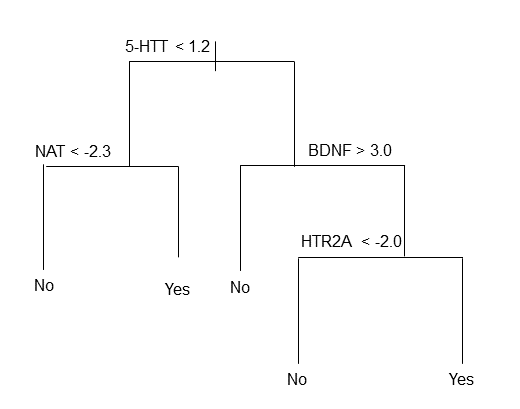
\includegraphics[width=12cm]{figures/decision_tree.png}
        \caption{A single decision tree in which drug-induced gene expression data are used to predict treatment effects}
        \label{fig:intr_tree}
      \end{figure}
      
      Figure \ref{fig:intr_tree} shows a single decision tree on fake drug expression data. In brief, for each time of splitting, we select a variable according to certain criteria and find a cutoff value of that variable to minimize the current loss. To grow a decision tree, the algorithm recursively splits the feature space of training data, and it stops when each leaf node has less than a minimum number of observations or the tree reaches the maximum depth. The \textit{Gini index}, a typical criterion used to make binary splits, measures the impurity of each node and is defined by \cite{james2013introduction}
      \begin{equation}
        G = \sum_{m=1}^T \sum_{k=1}^K  \hat{p_{mk}} (1 - \hat{p_{mk}}), 
      \end{equation}
      which measures total variance of binary classes for each leaf node. Here $T$ refers to the number of leaf nodes of a tree, $K$ denotes the number of classes, and $\hat{p_{mk}}$ represents the fraction of training observations in the mth region that are from the $k$th class. For binary classification $K$ is 2. 
      
      For tree-based regression, the procedure to grow a tree is similar to classification, but the criterion to make a binary split is different, which is \cite{james2013introduction}
      \begin{equation}
        \mathrm{EPE} = \sum_{m=1}^T \sum_{x_i \in r_m}  (y_i - \hat{y_{r_m}})^2, 
      \end{equation}

      Similarly, $T$ is the number of leaf nodes, $r_m$ is the $m$th leaf node, and $\hat{y_{r_m}}$ is the mean response of training observations in the $r_m$ region. Like linear models, penalty can also be imposed to reduce the complexity of tree to build models with lower variance. One form of regularization is to control the number of leaf nodes \cite{james2013introduction}:
      \begin{equation}
        G = \sum_{m=1}^T \sum_{k=1}^K \hat{p_{mk}} (1 - \hat{p_{mk}}) + \alpha T
      \end{equation}

      Note that in regression the average output of training observations falling into a leaf node can be regarded as the predicted value; in classification the probability of a class is estimated by the fraction of observations belonging to the class in the leaf node. 
      
      A single decision tree usually suffers from high variance which leads to poor predictive performance. Also, some observations may be predicted worse than others. To alleviate the problems of predicting with a single tree, “combining” many trees trained on different subsets of training data might improve predictive performances.Bagging, random forest, and boosting are powerful tools using this idea.
      
      Bagging, or bootstrap aggregation, is a procedure to reduce the variance of tree-based methods by averaging estimations from models trained on a number of training sets sampled by bootstrap. Observations are drawn with replacement in a bootstrap procedure. The prediction from bagging (for regression) is given by \cite{james2013introduction}
      \begin{equation}
        \hat{f}_{bag} (x) = \frac{1}{B} \sum_{b=1}^B \hat{f^{*b}}(x)
      \end{equation}
      where $B$ is the number of trees ensembled. For qualitative outputs, a majority vote can be taken to determine the predicted classes, i.e., the most commonly occurring class among the $B$ estimators for each observation.

      Random forest (RF) may be considered as a modified version of standard bagging. In random forest, only a subset of features is considered at each candidate split. Usually, features chosen for splitting are a minority of total features, and typically $m \approx \sqrt{p}$ (where p is the total number of features) is chosen in practice \cite{james2013introduction}. This aims to reduce the correlation between different trees, as aggregating many uncorrelated trees will benefit from a larger variance reduction than aggregating trees that are highly correlated.

      Gradient boosting is a general ML approach which aims at combining weak learners to produce an improved prediction model and is most often applied to decision trees \cite{friedman2001greedy}. Unlike bagging and random forest, boosting grows trees sequentially. In essence the algorithm tries to improve the model sequentially via fitting a learner to the residuals (or pseudo-residuals) from the previous model. Boosting for classification tree was first proposed by Freund and Schapire in \cite{freund1995desicion}, based on the idea of growing new trees by emphasizing more on observations poorly learned by previous trees. Friedman later developed a more general framework for boosting \cite{friedman2001greedy}.

      There are several advantages for tree-based methods. Firstly, decision tree mimics human decision processes and is relatively easy to interpret. For ensemble models, feature importance may be assessed by various means, for example improvement in the criterion for split (e.g., Gini index) and permutation importance in random forest, and the number of times a feature is used or total gain of splits using the particular feature in boosted trees. Also, tree-based models can handle qualitative and quantitative features and response with ease. In linear models, dummy variables are needed to handle qualitative features, but tree-based methods can absorb qualitative variable directly. Tree-based methods are also robust to outliers and model complex nonlinear relationships well.

    \subsubsection{Support Vector Machine}
      Support vector machine (SVM) is a typical maximum margin classifier that aims to separate different classes with a large "gap" \cite{cortes1995support}. By using the "kernel trick", SVM can map feature space from low dimensions to high, even infinite, dimensions, which makes problems that cannot be solved in low dimensions solvable.
      
      Here we will discuss SVM for classification only. We first assume that the data $(X, Y)$ is linearly separable and $Y \in \{-1, 1\} ^n$. Intuitively, we can model this problem as follows:
      \begin{equation}
        \min_{\gamma, w, b} \frac{1}{2} w^T w, s.t. y_i (w^T x_i + b) > 1, i = 1, \cdots, m
      \end{equation}
      
      Here $w$ denotes coefficients, $b$ stands for the intercept, and $s.t.$ in the equation is abbreviation of "subject to". This is a typical convex problem with linear restrictions, and it can be solved using convex optimization techniques. In reality, linear separable data is very rare, and SVM can also adapt to inseparable cases with nonlinear decision boundary. The reformulated equation is as follows:
      \begin{equation}
        \begin{split}
          & \min_{\gamma, w, b} \frac{1}{2} w^T w + C \sum_{i=1}^m \xi_i \\
           s.t. & y_i (w^T \phi (x_i) + b) > 1 - \xi_i, \xi_i > 0, i = 1, \cdots, m
        \end{split}
      \end{equation}

      Here, $\phi(xi)$ maps features $x_i$ from low to higher dimensions to capture nonlinear relationships; $\xi_i$ are slack variables that allows some observations to be on the wrong side; and $C$ controls the penalty of relaxing the functional margin. Figure \ref{fig:intr_svm} shows a hypothetical classification problem in which two observations fall into wrong sides after the introduction of slack variables.
      
      \begin{figure}[h]
        \centering
        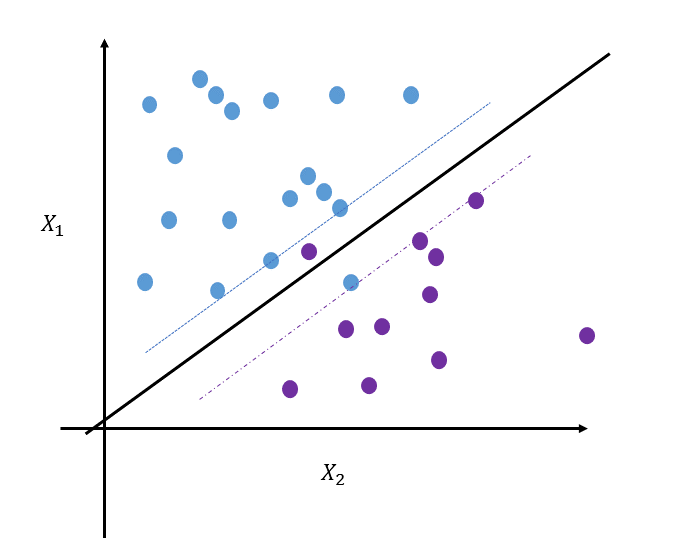
\includegraphics[width=10cm]{figures/SVM.png}
        \caption{A hypothetical classification task using linear SVM. Two observations fall into the wrong sides after the introduction of slack variables}
        \label{fig:intr_svm}
      \end{figure}

      The form of decision boundary can be transformed into the sum of inner product of feature mapped with the form of $\sum_{i=1}^m \alpha_i y_i \langle \phi(x_i), \phi(x) \rangle$, and $\langle \phi(x_i), \phi(x) \rangle$ is a kernel that measures the similarity between xi and x. The Gaussian (or radial basis function, RBF) kernel is one of the most widely used kernels to produce complex nonlinear decision boundaries. The Gaussian kernel can be expressed as: 
      \begin{equation}
        K(x, z) = \exp \bigg( - \frac{||x-z||^2}{2 \sigma^2} \bigg)
      \end{equation}

      There are serval key characteristics of SVM. First, the decision boundary of SVM is actually determined by observations near the boundary, and thus data points far away from the boundary have little effect on the decision boundary. It models nonlinear relationships well, and various kernels can be applied to make different complex decision boundaries to satisfy different classification problems \cite{bishop2006pattern}.

      SVM has been employed for drug or target discovery in earlier studies. For example, in a recent work, the authors integrated several layers of drug properties including chemical structures and proximity of targets in an interaction network and expression profiles and used SVM to predict therapeutic classes \cite{napolitano2013drug}. Another study adopted SVM trained on molecular structure, molecular activity, and phenotype data to discover new indications for drugs \cite{wang2013drug}. A study we mentioned earlier \cite{aerts2007pharmacological} employed SVM and DNN to learn drug therapeutic categories from gene expression data. Regarding the application of SVM on drug target discovery, studies \cite{bakheet2009properties,li2007prediction} utilized SVM on structural or chemical properties of known drug targets to identify promising drug targets.

      In our recent application, we used SVM with Gaussian kernel and found SVM in general performed favorably compared to other methods \cite{zhao2018drug}. We used the Python package "scikit-learn" \cite{pedregosa2011scikit,buitinck2013api} for implementation, but similar packages in R or other programming languages are also available.

      Regarding the limitations of this approach, SVM models are often difficult to interpret, and there is a lack of widely used criteria to quantify the importance of individual features. In the case of drug repositioning or target discovery, this may be a limitation given that we are usually interested in identifying which genetic or biological factors contribute to the treatment effects on diseases. As a kernel-based method, drug repositioning with SVM employs a comparable principle to other "similarity-based" approaches (e.g., a drug $X$ with high similarity to a known treatment A may also be able to treat the same disease) \cite{hodos2016silico}. Similarly, perturbation of a gene may induce a pattern of expression profile that is similar to that of a drug, then compounds acting on the gene may have similar mechanisms to the drug. Thus, one limitation is that such an approach may not be very good at revealing candidates with novel mechanisms of actions \cite{hodos2016silico}.

    \subsubsection{Deep Neural Networks}
      Deep learning has attracted increasing attention in recent years and contributed to significant advances in many fields such as computer vision. Deep neural networks (DNN) are based on the concept of  "representation learning" \cite{bengio2013representation} and are very good at capturing nonlinear relationships. Many different network architectures have been developed, but here we only discussed feedforward neural networks with fully connected layers.

      By using multiple hidden layers, DNN can handle more complex relationships than a simple single-layered network. The optimal number of hidden layers and neurons will depend on the nature and complexity of the problem as well as the data size. DNN usually requires relatively large sample sizes to achieve good predictive power as the number of parameters is large and overfitting can be a major problem. Dropout is a simple and widely used approach to avoid overfitting by “inactivating” a proportion of neurons randomly during training \cite{srivastava2014dropout}. Feature selection and shrinkage can also be applied by employing L1 and L2 regularization \cite{zou2005regularization}. There are also numerous other hyper-parameters to choose from, such as the activation function, learning rate, momentum, batch size, etc. For activation function of hidden layers, ReLU is often used. In the output layer, sigmoid function can be used in binary classification problems and softmax in multi-classification problems. The performance of DNN is promising in recent studies of drug repositioning and drug category classification \cite{aliper2016deep,zhao2018drug}. Nevertheless, DNN models are hard to interpret, and the choice of hyper-parameters is often difficult. The computational and time costs for training a model are relatively high (especially for large datasets); however, the use of graphic processing units (GPUs) can greatly accelerate the computing speed.

      With the rapid development of deep learning methodologies, they have been increasingly used for drug repurposing \cite{aliper2016deep,zhao2018drug,xie2017discovery} or prediction of various drug properties or toxicities. For example, Klambauer et al. applied deep neural networks on chemical features of compounds to predict their toxicities \cite{mayr2016deeptox}. Ryu et al. employed deep learning to improve prediction of drug-drug and drug-food interactions \cite{ryu2018deep}. Deep learning has also been used to predict synergistic effects of drugs in cancer therapy \cite{preuer2018deepsynergy}. Readers may also refer to recent reviews on the applications of deep learning in biomedicine and drug discovery \cite{baskin2016renaissance, chen2018rise, ching2018opportunities}.

    \subsubsection{Cross Validation to Assess Predictive Performance}
      Above we have introduced several common ML algorithms for training a prediction model. Meanwhile, assessing the performance of model is a critical issue, and the performance of the model in train set can dramatically underestimate of the true prediction error.
    
      To avoid overoptimistic estimation of model performance, the prediction error can be estimated in a new dataset independent of the training set, if such data is available. However, data is often limited, and a more popular approach is K-fold cross validation. A typical practice is to firstly split the entire dataset into K folds evenly and then set side onefold of data as testing set and train on the other folds in each loop. There is no fixed rule to determine K, but it is often set at 5 or 10. A very low K (e.g., leave-one-out cross validation) will lead to almost unbiased but high variance of the prediction error estimate, as the training sets are highly similar. Increasing K will reduce the variance but may increase the bias \cite{friedman2001elements}.
      
      In practice, one often needs to tune hyper-parameters, and dividing the data into training and testing sets will not be sufficient. In some studies, the authors would train the model in the training set and pick the hyper-parameters that give the best predictive performance in test set and then report the corresponding prediction error. (In case of cross validation, the "best" prediction error may be averaged over the K folds). However, such an approach still tends to give overoptimistic estimates of the prediction error as one is picking the best-performing parameters each time which may not be generalized to a completely new dataset \cite{varma2006bias}. To avoid this problem, the testing set should not be involved in parameter tuning. For example, the dataset can be divided into training, validation, and testing sets, in which the hyper-parameters are chosen based on predictive performance in the validation set. A more advanced approach is nested K-fold cross validation \cite{varma2006bias}. In this case, inner K-fold cross validation is used to choose the best hyper-parameters, and the performance of the model with the best parameters chosen is evaluated on the testing set.

    \subsubsection{Criteria for Model Selection}
      Here we describe criteria for assessing model fit and predictive performance. For regression, the most commonly used criteria are mean squared error loss. Below we discuss the metrics for classification.

      Log loss, or cross entropy, measures the negative log-transformed probability of belonging to expected class for each observation. Its equation is
      \begin{equation}
        \mathrm{EPE} = - \sum_i y_i \log p(x_i) + (1 - y_i) \log (1 - p(x_i)).
      \end{equation}
      Therefore, the higher the probability an observation belongs to the expected class, the smaller the log loss value of the observation. Cross entropy is a widely used objective function in classification tasks.

      If there is a predefined specific threshold to define a positive or negative outcome (e.g., say it is generally agreed that predicted probability $> 30$\% represents positive outcome), different measures such as sensitivity (aka recall), specificity, precision (aka positive predictive value), and F1 score (harmonic mean of precision and sensitivity) can be computed accordingly. However, often we may not have such a predefined threshold, and we may wish to consider the overall performance of the model under a variety of possible thresholds. In this case we may use the area under the receiver operating characteristic (ROC) curve (AUROC) or area under the precision-recall curve (AUPRC) as metrics of predictive performance.
      
      The ROC curve records the true positive rate (sensitivity) against false positive rate (1- specificity) at different thresholds. Area under the ROC curve (AUROC) is a commonly used metric to assess predictive performance especially in the medical field. For problems with class imbalance, it has been argued that AUPRC may better reflect the model performance \cite{davis2006relationship}.

    \subsubsection{Common Issues of Machine Learning in Biomedical Studies}
      Overfitting refers to overlearning of a model on the training data, leading to poor performance when applied in a new situation. Underfitting describes an opposite phenomenon, in which the model fails to capture the complex relationships within the data. A closely related concept is the “bias-variance” tradeoff. In general, models that are complex will have small bias but higher variance, while simpler models enjoy lower variance but have increased bias. Several approaches may be employed to reduce the risk of overfitting. For example, one may reduce the number of features by preselection or some form of dimension reduction, apply heavier regularization penalty to make the model simpler, or switch to less complex ML models. If possible, obtaining larger sample sizes will also alleviate the problem. Underfitting can be overcome by opposite strategies. 
      
      However, how do we know whether a model overfits or underfits in practice? A typical strategy is to examine or plot a curve of the training and testing errors. If training error is unacceptably high and the gap between the two errors is small, then the complexity of the model chosen may be too low, or underfitting is present. If the training error is close to 0 but testing error is high, the model might be overfitting.

      Imbalanced data is a problem often encountered in biomedical applications in which observations with positive outcome may be uncommon. For example, only a few people may develop a disease or complication, or only a minority of the drugs can treat a specific disorder. There are several common strategies for imbalanced data, such as down-sampling the majority class, up-sampling of the minority class, and constructing new cases by methods such as SMOTE \cite{chawla2002smote}. Here we briefly describe how to tackle this problem with class weights. If the default weight for each observation is 1 and positive observations are rare, the total weights of positive and negative observations will be imbalanced. To remedy the situation, we can \textit{increase} the weight for each positive observation to balance the total weights of the positive and negative classes. This strategy can also be used in multi-class classification problems. In a recent work of drug repositioning, we did observe obvious improvement in predictive power using the above weighting scheme \cite{zhao2018drug}.

  \section{Machine Learning Methods for ITE Estimation}
    Machine learning is a data-driven approach, without strong modeling assumptions, and techniques such as cross validation and various penalties can be incorporated to avoid overfitting, reducing the possibility of false discovery. There is also a rise in the number of studies using machine learning approach to estimate ITE. typically, there are two typical steps in estimation of heterogeneous treatment effects. We need to identify groups of heterogeneity in treatment effects firstly, and then to estimate of individual treatment effects, ie, individual risk prediction \cite{scarpa2019assessment}. The are mainly two streams in application of machine learning approaches to ITE estimation: averaged treatment effect of subgroups defined by learning algorithms and ensembled approaches based on tree-based methods.
    
    Some of recent studies focus on detecting subgroups of heterogeneity in treatment effects. Specifically, these studies try to to estimate the difference of averaged outcome between treatments and controls in pre-specified subgroups \cite{gail1985testing} or subgroup defined by learning algorithms \cite{su2009subgroup, su2011interaction, athey2016recursive,foster2011subgroup, lipkovich2011subgroup}. Su et. al. employed interaction tree to iteratively searching subgroups based on treatment effect \cite{su2009subgroup,su2011interaction}. Similarly, causal trees proposed by Athey and Imbens estimate the treatment effect at the leaves of the tree \cite{athey2016recursive}. However, the definition of subgroup is arbitrary and somewhat algorithm dependent, the generality of subgroup algorithms maybe poor, and these subgroup algorithms tend to over-estimate the heterogeneity present. As stated in the study \cite{wager2018estimation}, the impediment of iteratively searching for subgroups present obvious treatment effect and reporting only the results for subgroups with extreme treatment effects to highlight heterogeneity may be highly spurious. In the high dimensional setting, it's still very challenging to divide subjects into appropriate subgroups \cite{powers2017some}. It's the same case for genomic data. 

    Forests-based methods have gained popularity in ITE estimation in the past years \cite{wager2018estimation,kunzel2019metalearners,lu2018estimating,dasgupta2014risk,hill2013assessing,hill2013assessing,green2012modeling}, because forests-based methods have very nice features. Most importantly, they have excellent interpretability since variables contributing to prediction can be extracted, and even can visualize the procedure of decision-making by plotting some important trees. Forests-based methods capture complex interactions in data. A study shows that forests-based methods can discover predictive and stable high-order interactions \cite{basu2018iterative}. They also has other benefits, like less likely to overfit and robust to missing values. Studies \cite{green2012modeling,hill2011bayesian, hill2013assessing} employs bayesian forest-based methods to estimate heterogeneous treatment effects, which are based on Bayesian additive regression tree (BART) method \cite{chipman2010bart}. One advantage of this kind of approach is that reliable intervals for treatment effects can be readily obtained by MCMC sampling. Some other methods in frequentist form, like Meta learners and deep learning based, for ITE estimation could be found in \cite{kunzel2019metalearners,johansson2016learning,powers2017some}. Powers et al. proposed causal boosting, causal Multivariate adaptive regression splines (MARS) and pollinated transformed outcome (PTO) forests to fit adjusted outcomes \cite{powers2017some}. Another study employed deep learning to make counterfactual inference on ITE \cite{johansson2016learning}. In practice, these approaches try to fit $\mu_1(\mathbf{x})$ and $\mu_0(\mathbf{x})$ simultaneously / separately and estimate the difference by computing the different between $\mu(\mathbf{x},w)$ and $\mu(\mathbf{x}, 1-w)$.  Similarly, metaalgorithms decompose estimation of the CATE into several sub-regression tasks, that can be tackled with any supervised learning method \cite{kunzel2019metalearners}. A limitation of these studies is lack of formal statistical inference results \cite{wager2018estimation}. Wager et al. proposed causal forests with honest to estimate ITE \cite{wager2018estimation}. In causal forests with honest, training set is splited into two parts, one partition is used for tree growing, and the other partition is utilized to make honest estimation; Moreover, the authors have showed that causal forests with honest have good asymptotic properties \cite{wager2018estimation}.
  
  \section{Summary}
    In this section, we introduced the current situation of drug development and difficulties in the process of developing a new medication, reviewed some studies using computational approaches to drug target discovery and purposing, and discussed their limitations. As the technique behind the computational method largely belongs to the field of machine learning, we gave a detailed introduction of machine learning approaches, with some biomedical applications of corresponding ML methods as examples. Then we went into a more clinically relevant topic of discovering ITE. For estimation of ITE, we focused on methods discovering ITE using machine learning based approaches, reviewed some relevant studies based on ML approaches, and pointed out possible limitations of these studies.
     
\chapterend
% % chapter background study
\chapter{Background Study}


\chapterend

\chapter{Drug Repurposing}
\label{chap:Repurposing}

\section{Background}
  \subsection{Motivation}
    Development of new medications is a very lengthy and costly process. While investment in research and development has been increasing, there is a lack of proportional rise in the number of drugs approved in the past two decades, especially for drugs with novel mechanisms of actions \cite{pammolli2011productivity}. There is an urgent need for innovative approaches to improve the productivity of drug development. This is particularly true for some areas like psychiatry, for which there has been lack of therapeutic advances for some time \cite{krystal2014psychiatric,hyman2013psychiatric}.
    
    Finding new indications for existing drugs, an approach known as drug repositioning or repurposing, can serve as a useful strategy to shorten the development cycle \cite{dudley2011exploiting}. Repurposed drugs can be brought to the market in a much shorter time-frame and at lower costs. With the exponential growth of “omics” and other biomedical data in recent years, computational drug repositioning provides a fast, cost-effective and systematic way to identify promising repositioning opportunities \cite{dudley2011exploiting}.  

    In this study we describe a general drug repositioning approach by predicting drug indications based on their expression profiles, with a focus on applications in psychiatry. We treat drug repositioning as a supervised learning problem and apply different state-of-the-art machine learning methods for prediction. Drugs that are not originally indicated for the disease but have high predicted probabilities serve as good candidates for repositioning. There are several advantages of this approach. Firstly, the presented approach is a general and broad framework that leverages machine learning (ML) methodologies, a field with very rapid advances in the last decade. This provides great flexibility and opportunities for further improvement in the future as virtually any supervised learning methods can be applied. Newly developed prediction algorithms can also be readily incorporated to improve the detection of useful drug candidates. In addition, the method described here is widely applicable to any chemical or drugs with expression profiles recorded, even if the drug targets or mechanisms of actions are unknown. For example, herbal medicine products may contain a mixture of ingredients with uncertain drug targets; even for many known medications (e.g. lithium \cite{malhi2013potential}), their mechanisms of actions and exact targets are not completely known. If transcriptomic profiling has been performed, they can still be analyzed for therapeutic or repositioning potential under the current approach.

  \subsection{Related Works}
    There has been increasing interest in computational drug repositioning recently, in view of the rising cost of new drug development. Hodos et al. \cite{hodos2016silico} provided a comprehensive and updated review on this topic. Similarity-based methods (e.g. ref. \cite{gottlieb2011predict,oh2014network,liu2015similarity,luo2016drug,napolitano2013drug,li2012new}) represent one common approach, but as noted by Hodos et al., the dependence on data in the “nearby pharmacological space” might limit the ability to find medications with novel mechanisms of actions. Another related methodology is the network-based approach \cite{lotfi2018review}, which typically requires data on the relationship between drugs, genes and diseases as well as connections within each category (e.g. drug-drug similarities). It can integrate different sources of information but may still be constrained by the focus on a nearby pharmacological space and the choice of tuning parameters in network construction or inference is often ad hoc \cite{hodos2016silico}. The present work is different in that we apply a broad framework for repositioning and we do not focus on one but many different kinds of learning methods. There is comparatively less reliance on known drug mechanisms or the “nearby pharmacological space” as we let the different algorithms “learn” the relationship between drugs, genes and disease in their own ways. We note that kernel-based ML methods such as support vector machine (SVM) are also based on some sort of similarity measures. A related work \cite{napolitano2013drug} have also examined SVM as a promising ML approach for drug repositioning and identified several interesting candidates. However, here our focus is different in that we considered a variety of other approaches and SVM is one of the methods which falls under the broader framework of ML for repositioning. We also employed more in-depth validation strategies, such as assessing enrichment for drugs considered in clinical trials and correlations with the level of literature support. As for other advantages of ML approaches, for high-throughput omics data, often only a subset of genes or input features are relevant, and many ML methods are able to “learn” which features to consider for repositioning. As we shall discuss later, ML approaches may also provide a new avenue to explore the mechanisms of different drug classes, by studying the variable importance of gene features.

    We are particularly interested in drug repositioning for psychiatric disorders in view of the lack of novel treatments in the area. Although computational drug repositioning has attracted increased attention recently, relatively few studies focus on psychiatric disorders (except e.g. \cite{xu2015phenopredict,de2016gene,powell2017transcriptomic,so2017analysis}), compared to other areas like oncology. Psychiatric disorders are leading causes of disability worldwide \cite{vigo2016estimating}, however there have been limited advances in the development of new pharmacological agents in the last two decades or so \cite{hyman2013psychiatric}. Development of new therapies is also limited by the difficulty of animal models to fully mimic human psychiatric conditions \cite{nestler2010animal}. Investment by drug companies has in general been declining \cite{hyman2013psychiatric}, and new approaches for drug discoveries are very much needed in this field. We will explore repositioning opportunities for schizophrenia along with depression and anxiety disorders. Here depression and anxiety disorders are analyzed together as they are highly clinically comorbid \cite{lamb2006connectivity,kessler2015anxious}, show significant genetic correlations \cite{otowa2016meta}, and share similar pharmacological treatments \cite{ballenger2000anxiety}. 
    
  \subsection{Significances}
    Contributions of this study are summarized below. Firstly, we presented a general workflow and approach to drug repositioning of a disease based on ML methods, leveraging drug expression profiles as predictors. While previous work \cite{aliper2016deep} has also proposed the use of ML on drug transcriptome profiles for classifying drugs into groups (e.g. anti-cancer drugs, cardiovascular drugs, drugs acting on the central nervous system etc.), we focused on drug repositioning for particular diseases instead of predicting the big therapeutic groups, as disorders in the same group can have diverse treatments. Secondly, we have performed a comparison of the predictive performances of five state-of-the-art and perhaps most commonly employed ML algorithms, including deep neural networks, support vector machines, elastic net, random forest and gradient boosted trees. Thirdly, we identified new repositioning opportunities for schizophrenia and depression/anxiety disorders and validated the relevance of the repositioned drugs by showing their enrichment among drugs considered for clinical trials, as well as support by previous literature. As another means of validation, we also showed that the predicted probabilities of treatment potential are significantly and positively correlated with the level of literature support (using the number of research articles support as proxy). Finally, we explored which genes and pathways contributed the most to our predictions, hence shedding light on the molecular mechanisms underlying the actions of antipsychotics and antidepressants. 

\section{Datasets and Methods}
  \subsection{Datasets}
    We present a general drug repositioning approach adopting a supervised learning approach. We construct prediction models in which the outcome is defined as whether the drug is a known treatment for the disease, and the predictors are expression profiles of each drug. Drugs that are not originally known to treat the disease but have high predicted probabilities are regarded as good candidates for repositioning.

    \subsubsection{Drug expression data}
      The expression data is downloaded from Connectivity Map (CMap), which captures transcriptomic changes when three cell lines (HL60, PC3, MCF7) were treated with a drug or chemical \cite{lamb2006connectivity}. We downloaded raw expression data from Cmap, and performed normalization with the MAS5 algorithm \cite{pepper2007utility}. Expression levels of genes represented on more than one probe sets were averaged. We employed the limma package \cite{ritchie2015limma} to perform analyses on differential expression between treated cell lines and controls. Analyses were performed on each combination of drug and cell line, with a total of 3478 instances. Note the expression of each drug was measured on three different cell lines. Expression measurements were available for 12436 genes. Thus, the scale of our dataset is 3478×12436. Statistical analyses were performed in R3.2.1 with the help of the R package "longevityTools".

    \subsubsection{Defining drug indications}
      Drug indications were extracted from two known resources, namely the Anatomical Therapeutic Chemical (ATC) classification system and the MEDication Indication Resource high precision subset (MEDI-HPS)\cite{kuhn2016sider}. We focus on schizophrenia as well as depression and anxiety disorders in this study. From the ATC classification system, two groups of drugs were extracted, consisting antipsychotics and antidepressants. On the other hand, the MEDI-HPS dataset integrates four public medication resources, including RxNorm, Side Effect Resource 2 (SIDER2) \cite{kuhn2016sider}, Wikipedia and MedlinePlus. We used the MEDI high-precision subset (MEDI-HPS) which only include drug indications found in RxNorm or in at least 2 out of 3 other sources \cite{wei2013development}. This subset achieves a precision of up to 92\% according to Wei et al. \cite{wei2013development}. To our knowledge, antidepressants from ATC and depression / anxiety from MEDI-HPS roughly fall into the same category, and this is also the same for antipsychosis from ATC and schizophrenia from MEDI-HPS. 

  \subsection{Methods}
    We employed different state-of-the-art machine learning approaches including deep neural networks (DNN) \cite{goodfellow2016deep}, support vector machine (SVM) \cite{cortes1995support}, random forest (RF) \cite{breiman2001random}, gradient boosted machine with trees (GBM) \cite{friedman2001greedy} and logistic regression with elastic net regularization (EN) \cite{zou2005regularization} to predict indications with binary classifiers. Our data is imbalanced as only a minority of the drugs are indicated for schizophrenia or depression/anxiety disorders. We performed both unweighted and weighted analyses in this study; in the weighted analysis, class weights are adjusted such that the minority group (drugs indicated for the disorder) will receive higher weight to achieve a balance between positive and negative instances. 

    In our unweighted model, DNN was implemented in the python package keras. We employed a fully connected feedforward neural network. Hyperparameters were chosen by the "fmin" optimization algorithm from "hyperopt", which employs a sequential model-based optimization approach \cite{bergstra2013hyperopt}. The tree-structured Parzen estimator (TPE) was used. The more sophisticated hyper-parameter search strategies provided by sequential model-based methods may produce better results than simpler approaches (e.g. grid search) when the number of hyper-parameters is large, such as in deep learning settings \cite{bergstra2013hyperopt}. Fifty evaluations were run for each search of optimal hyper-parameters. Dropout and mixed $L1/L2$ penalties were employed to reduce over-fitting. The neural networks consisted of two or three layers, with number of nodes selected uniformly from the range [64, 1024]. Dropout percentage was selected uniformly from [0.25, 0.75], and $L1/L2$ penalty uniformly from [1E-5, 1E-3]. Optimizer was chosen from "adadelta" \cite{zeiler2012adadelta}, "adam" \cite{kingma2014adam} and "rmsprop" \cite{hinton2012neural}, and the activation function chosen from "relu", "softplus" or "tanh". One hundred epochs were run for each model and we extracted the model weights corresponding to the best epoch. 
    
    We also attempted "hyperopt" for the weighted analysis, however the predictive performance was unexpectedly poor due to unclear reasons yet to be revealed. We therefore turned to hyperparameter selection with grid search, with some adjustments in the parameter ranges. A two-layer neural network was constructed with dropout and mixed $L1/L2$ to avoid over-fitting. The number of neurons in the first hidden layer was selected from \{1000, 1500, 2000\}, the number in the second layer from \{500, 1000, 1500\}, dropout rate from \{0.4, 0.5, 0.6, 0.7, 0.8\}, $L1/L2$ penalty from intervals [-13, -3] and [-9, -8] in log space and the number of epochs from [10, 20, 30, 50]. In order to speed up hyperparameter selection, we first chose the number of epochs, the best optimizer and activation function (following the same parameter range as described above) with other parameters fixed, and then used the best parameters chosen in the first step to find the optimal complexity of our neural networks by selecting the number of neurons in each layer, dropout and mixed $L1/L2$ penalties.

    SVM, RF and GBM models were implemented in "scikit-learn" (sklearn) in python. Hyper-parameter selection was performed by the built-in function GridSearchCV in sklearn. For SVM, we chose radial basis function as the kernel. The two hyper-parameters $C$ and $\gamma$ were selected from [-5, 2] and [-6, 2] in $\log$10-space respectively. 
    
    For RF, the number of bagged trees was set to 1000, the maximum number of features used for splitting was selected from \{800, 1000, 1500, 2000, 3000, 5000 \} and min\_samples\_leaf (the minimum number of samples required at a leaf node) was selected from \{1, 3, 5, 10, 30, 50, 80 \}. For GBM, the number of boosting iterations was selected from a sequence of 100 to 1001 with step size 50, learning rate from \{0.005, 0.01, 0.015, 0.02, 0.03, 0.05 \}, subsampling proportion from \{0.8, 1 \}, maximum depth of each estimator from \{2, 3, 5, 10\} and maximum number of features from \{10, 30, 50, 100, 500, 1000 \}. Finally, the EN model was implemented by the R package "glmnet" \cite{friedman2010regularization}. The elastic-net penalty parameter $\alpha$ was chosen from seq(0, 1, by=0.1), with other settings following the default.

    \subsubsection{Nested Cross-validation}
      We adopted nested three-fold cross validation (CV) to choose hyper-parameters and evaluate model performances. It has been observed that optimistic bias will result if one uses simple CV to compute an error estimate for a prediction algorithm that itself is tuned using CV \cite{varma2006bias}. Nested CV avoids this problem and is able to give an almost unbiased estimate of prediction accuracy \cite{varma2006bias}. The inner loop CVs were used to choose the parameters that optimized predictive performance. In each outer loop CV we made predictions on the corresponding test set using the best model trained from the inner CV loops. To achieve maximum consistency in our comparisons, we compared different methods on the same test set in each loop. Note that the test sets were not involved in model training or parameter tuning.

    \subsubsection{Predictive performance measures}
      The performances of the machine learning methods were evaluated in the test sets using three metrics, including log loss, area under the receiver operating characteristic curve (ROC-AUC) and area under the precision recall curve (PR-AUC). Log loss compares the predicted probabilities against the true labels. The receiver operating characteristic curve, which plots the sensitivity (i.e. recall) against (1- specificity), is a very widely used approach to evaluate predictive performances in biomedical applications. The precision-recall curve on the hand plots the precision (i.e. positive predictive value) against the sensitivity (recall). Since precision depends on the overall proportion of positive labels, the PR-AUC is also dependent on such proportions. Davies et al. \cite{davis2006relationship}  that the PR curve may give more informative comparisons when working with imbalanced data.

    \subsubsection{Identifying important genes and pathways}
      We also performed analyses to reveal the genes which contribute the most to the prediction model. For elastic net, we extracted the genes with non-zero coefficient in at least one cross-validation fold, and the resulting genes were subject to an over-representation analysis (ORA) (using hypergeometric tests) to reveal the pathways involved. For RF and GBM, feature importance was computed using built-in functions in sklearn based on Gini importance (i.e. the average decrease in node impurity). We then performed a gene-set enrichment analysis (GSEA \cite{subramanian2005gene}) based on the genes together with their respective importance scores (the highest score across three folds was taken). For SVM and DNN, there is a lack of widely adopted importance measures, so we focused on the rest of ML methods in this part. Pathway analyses were conducted by the web-based program WebGestalt \cite{wang2017webgestalt}. Four pathway databases were considered in our analyses, including KEGG, PANTHER, Reactome and Wikipathways.
    
    \subsubsection{External validation by testing for enrichment of psychiatric drugs considered for clinical trials}
      We then performed additional analyses to assess if the drugs with high predicted probabilities from our machine learning models are indeed good candidates for repositioning. Briefly, we tested whether the drugs with no known indication for the disease but high predicted probabilities are more likely to be included in clinical trials. 

      In the first step, we filtered off drugs that are known to be indicated for the disease as derived from ATC and MEDI-HPS. This is because we are mainly interested in repositioning other drugs of unknown therapeutic potential, and that the labels of drug indication (from ATC or MEDI-HPS) have already been utilized in the ML prediction steps. Including known indications will lead to over-optimistic estimates of significance of enrichment. Next, we extracted a list of drugs that were included in clinical trials for schizophrenia as well as depression and anxiety disorders. The list was derived from clincialTrial.gov and we downloaded a pre-compiled version from.

      We then tested for enrichment of those drugs listed in clinicalTrial.gov among the top repositioning results. We performed an enrichment analysis of “drug-sets”, similar to a gene-set analysis approach widely used in bioinformatics \cite{de2016gene}. We performed one-tailed t-tests to assess if the predicted probabilities (derived from machine learning models) are significantly higher for psychiatric drugs considered in clinical trials.

    \subsubsection{Searching for literature support}
      We manually search for literature support for the top 15 repositioning hits for each method in PubMed and Google scholar. The search strategy is given in Supplementary text. A limitation of manual search is that it is extremely time-consuming to perform such a search for all drugs. It should be noted that publication bias is likely to be present (as negative studies are less likely to be reported), although it is difficult to exactly quantify the extent of bias. As we shall discuss later, we did find literature support for a number of top repositioning candidates, but it is still possible that similar evidence may be found for drugs ranked in the middle or lower. Also, one may wish to assess whether drugs with less (or no) support by prior studies would indeed have lower predicted probabilities (similar to having ‘negative controls’ in an experiment). 

      To ensure an unbiased and more comprehensive comparison, we conducted an analysis with "automated" literature mining on all drugs in PubMed. We extracted the number of research articles supporting each drug’s association with the corresponding psychiatric disorder (schizophrenia or depression/anxiety). We then examined the correlation between the number of research articles support and the predicted probabilities of treatment potential from ML models. Similar approaches for validating repositioning candidates based on literature mining have also been used in other studies \cite{huang2014drugcomboranker}. As the number of articles is typically skewed and not normally distributed, we employed Spearman and Kendall correlation measures. We also compared the predicted probabilities of drugs with no article support versus those with at least one article support. We hypothesized that drugs without any literature support would have lower predicted probabilities from ML models, and vice versa. We used the Wilcoxon rank-sum test for such comparison. All tests were carried out in R 3.2.3 and the tests were one-tailed. Similar to the enrichment test discussed above, drugs that are known to be indicated for the disorder (from ATC or MEDI-HPS) were excluded from this analysis. This is because the indication label of these drugs have been used in the ML model, which may lead to over-optimistic results, and that we wish to focus on repositioning potential of other drugs of unknown significance.

\section{Experiment Results}
  \subsection{Predictive performance comparison}
    \subsubsection{Unweighted analysis }

      \begin{table}[htbp]
        \centering
        \begin{threeparttable}
        \caption{Average predictive performance of different ML models across four datasets in unweighted (top) and weighted analysis (bottom)}
          \begin{tabular}{c|cccc}
          \toprule
          \textbf{Unweighted} & \multicolumn{4}{c}{Average Log Loss} \\
          \textbf{ analysis} & MEDI-HPS DEP/ANX & ATC ATD  & MEDI-HPS SCZ  & ATC ATP  \\
          \midrule
          SVM   & \textbf{0.1188} & 0.0943 & \textbf{0.1018} & \textbf{0.0895} \\
          EN    & 0.1249 & \textbf{0.0916} & 0.1097 & 0.0954 \\
          DNN   & 0.124 & 0.0948 & 0.1111 & 0.0992 \\
          GBM   & 0.1293 & 0.1018 & 0.1157 & 0.1039 \\
          RF    & 0.1294 & 0.1002 & 0.1155 & 0.1013 \\
                & \multicolumn{4}{c}{\textit{Average ROC-AUC}} \\
          SVM   & \textbf{0.7141} & 0.7619 & \textbf{0.7705} & \textbf{0.7755} \\
          EN    & 0.725 & \textbf{0.779} & 0.7515 & 0.7681 \\
          DNN   & 0.6952 & 0.7456 & 0.7533 & 0.7604 \\
          GBM   & 0.6536 & 0.6042 & 0.7172 & 0.7433 \\
          RF    & 0.6315 & 0.639 & 0.7036 & 0.7501 \\
                & \multicolumn{4}{c}{\textit{Average PR-AUC}} \\
          SVM   & \textbf{0.2026} & \textbf{0.1485} & \textbf{0.2973} & \textbf{0.3379} \\
          EN    & 0.1372 & 0.1008 & 0.1586 & 0.2087 \\
          DNN   & 0.1447 & 0.0877 & 0.1577 & 0.2156 \\
          GBM   & 0.091 & 0.0417 & 0.1426 & 0.1528 \\
          RF    & 0.1193 & 0.0639 & 0.1677 & 0.1703 \\
          \midrule
          \textbf{weighted} & \multicolumn{4}{c}{Average Log Loss} \\
          \textbf{ analysis} & MEDI-HPS DEP/ANX & ATC ATD  & MEDI-HPS SCZ  & ATC ATP  \\
          \midrule
          SVM   & \textbf{0.1189} & \textbf{0.0934} & \textbf{0.1022} & \textbf{0.0898} \\
          EN    & 0.5803 & 0.5344 & 0.5028 & 0.5112 \\
          DNN   & 0.1309 & 0.099 & 0.1308 & 0.1098 \\
          GBM   & 0.1281 & 0.1032 & 0.1114 & 0.0981 \\
          RF    & 0.1234 & 0.0943 & 0.106 & 0.0939 \\
                & \multicolumn{4}{c}{\textit{Average ROC-AUC}} \\
          SVM   & 0.7198 & 0.7718 & 0.7731 & 0.7765 \\
          EN    & 0.661 & 0.7394 & 0.7494 & \textbf{0.7997} \\
          DNN   & \textbf{0.7424} & \textbf{0.7979} & 0.741 & 0.7576 \\
          GBM   & 0.7155 & 0.7578 & 0.7584 & 0.7794 \\
          RF    & 0.689 & 0.7355 & \textbf{0.7843} & 0.7801 \\
                & \multicolumn{4}{c}{\textit{Average PR-AUC}} \\
          SVM   & \textbf{0.2017} & \textbf{0.151} & \textbf{0.298} & \textbf{0.3361} \\
          EN    & 0.0751 & 0.0896 & 0.152 & 0.203 \\
          DNN   & 0.1796 & 0.1107 & 0.2278 & 0.2641 \\
          GBM   & 0.18  & 0.1168 & 0.2697 & 0.278 \\
          RF    & 0.1771 & 0.1165 & 0.2721 & 0.2707 \\
          \bottomrule
          \end{tabular}%
          \begin{tablenotes}
            \small
            \item 1. Values of evaluation metrics for algorithms with the best performance in each dataset (for each evaluation metrics) are marked in bold. 
            \item 2. SVM: support vector machines; EN: logistic regression with elastic net regularization; DNN: deep neural networks; RF: random forest; GBM, gradient boosted machines. 
            \item 3. MEDI-HPS: MEDication Indication - High Precision Subset; ATC: Anatomical Therapeutic Chemical classification. 
          \end{tablenotes}
        \end{threeparttable}  
        \label{tab:repurposing_ml_result}%
      \end{table}%

      The average predictive performances (averaged over three folds) of different machine learning methods are listed in Table \ref{tab:repurposing_ml_result}. When considering log loss as the criteria of interest, SVM gave the best result overall, though EN showed the best performance in one of the four datasets. DNN and EN showed quite similar predictive performances. RF and GBM were slightly worse than other methods, but the difference was small. 
      When ROC-AUC was considered as the performance metric, SVM and EN gave similar performances. SVM outperformed EN in the schizophrenia datasets, while EN showed better results in the other two datasets. The performance of DNN was worse than that of SVM and EN, although the differences were not large. The two tree-based methods performed worse especially in the depression/anxiety datasets.
      We then considered PR-AUC, which is more sensitive to imbalanced data, as the measure of predictive performance. SVM was the best-performing method. EN and DNN followed with very similar performances. Consistent with other performance measures, GBM and RF did not perform as well in the depression/anxiety datasets, but the performance was more comparable for the schizophrenia datasets.

    \subsubsection{Weighted analysis} 
      Compared with unweighted analysis, we observed improvements in predictive performance for several methods including GBM, RF and deep learning. SVM and EN performed similarly in general. Considering ROC-AUC, deep learning performed the best for depression and anxiety disorders, while RF and EN showed highest ROC-AUC for schizophrenia. SVM achieved the best PR-AUC and log-loss compared to other ML approaches.

      \begin{table}[htbp]
        \centering
        \caption{Enrichment for psychiatric drugs included in clinical trials among the repositioning hits}
        \begin{threeparttable}
          \begin{tabular}{cccc}
          \toprule
                & \multirow{2}[4]{*}{Dataset} & unweighted analysis & weighted analysis \\
      \cmidrule{3-4}          &       & P-value & P-value \\
          \midrule
          \multirow{4}[1]{*}{SVM} & MEDI-HPS DEP/ANX & \textbf{0.0014} & \textbf{0.0011} \\
                & ATC ATD & \textbf{0.018} & \textbf{0.0039} \\
                & MEDI-HPS SCZ  & \textbf{0.0205} & \textbf{0.0264} \\
                & ATC ATP & \textbf{0.0098} & \textbf{0.0084} \\
          \midrule
          \multirow{4}[0]{*}{EN} & MEDI-HPS DEP/ANX & \textbf{0.0022} & \textbf{0.0023} \\
                & ATC ATD & \textbf{0.0032} & \textbf{0.0087} \\
                & MEDI-HPS SCZ  & \textbf{0.0294} & \textbf{0.0315} \\
                & ATC ATP & \textbf{0.0104} & \textbf{0.0033} \\
          \midrule
          \multirow{4}[0]{*}{DNN} & MEDI-HPS DEP/ANX & \textbf{0.0105} & \textbf{0.0009} \\
                & ATC ATD & 0.1369 & \textbf{0.0017} \\
                & MEDI-HPS SCZ  & 0.0908 & \textbf{0.019} \\
                & ATC ATP & \textbf{0.0237} & \textbf{0.0021} \\
          \midrule
          \multirow{4}[0]{*}{GBM} & MEDI-HPS DEP/ANX & \textbf{0.0494} & \textbf{0.0003} \\
                & ATC ATD & \textbf{0.0433} & \textbf{0.0002} \\
                & MEDI-HPS SCZ  & 0.2283 & \textbf{0.0269} \\
                & ATC ATP & 0.2482 & \textbf{0.0005} \\
          \midrule
          \multirow{4}[1]{*}{RF} & MEDI-HPS DEP/ANX & 0.0651 & \textbf{0.0005} \\
                & ATC ATD & 0.2518 & \textbf{0.0007} \\
                & MEDI-HPS SCZ  & 0.1299 & \textbf{0.0427} \\
                & ATC ATP & 0.5232 & \textbf{0.0063} \\
          \bottomrule
          \end{tabular}%
          \begin{tablenotes}
            \item P-values $< 0.05$ and with FDR less than 0.05 are in bold.
          \end{tablenotes}
        \end{threeparttable}
        \label{tab:repurposing_enrichment}%
      \end{table}%

  \subsection{Enrichment for psychiatric drugs considered clinical trials}
    We further tested whether the top repositioning results are enriched for drugs included in clinical trials for psychiatric disorders. As shown in Table \ref{tab:repurposing_enrichment}, we observed significant enrichment of such drugs for both schizophrenia and depression/anxiety disorders across all methods in the weighted analysis. In addition, most results in the unweighted analysis were also significant. This external validation provides further support to the usefulness of our approach in identifying new repositioning opportunities.
    
    \begin{table}[htbp]
      \centering
      \caption{Correlations between predicted probability of treatment potential with number of research articles supporting association with schizophrenia or depression/anxiety}
      \begin{threeparttable}
        \begin{tabular}{ccccc}
        \toprule
              & MEDI-HPS  DEP/ANX & ATC ATD & MEDI-HPS SCZ & ATC ATP \\
        \midrule
              & \multicolumn{4}{c}{Spearman's rho} \\
        SVM   & \textbf{0.078} & 0.049 & \textbf{0.098} & 0.088 \\
        EN    & 0.031 & 0.043 & 0.091 & 0.073 \\
        DNN   & 0.075 & \textbf{0.065} & 0.085 & \textbf{0.11} \\
        GBM   & 0.065 & 0.05  & 0.082 & 0.102 \\
        RF    & 0.066 & 0.051 & 0.052 & 0.055 \\
        \midrule
              & \multicolumn{4}{c}{Kendall's tau} \\
        SVM   & \textbf{0.06} & 0.037 & \textbf{0.077} & 0.068 \\
        EN    & 0.024 & 0.033 & 0.071 & 0.058 \\
        DNN   & 0.058 & \textbf{0.05} & 0.067 & \textbf{0.086} \\
        GBM   & 0.05  & 0.038 & 0.064 & 0.08 \\
        RF    & 0.052 & 0.04  & 0.041 & 0.044 \\
        \midrule
              & \multicolumn{4}{c}{Spearman correlation p-value} \\
        SVM   & \textbf{2.09E-05} & 4.91E-03 & \textbf{6.46E-09} & 1.47E-07 \\
        EN    & 4.89E-02 & 4.91E-03 & 5.96E-08 & 9.16E-06 \\
        DNN   & 3.45E-05 & \textbf{2.64E-04} & 3.37E-07 & \textbf{7.53E-11} \\
        GBM   & 2.91E-04 & 3.87E-03 & 9.64E-07 & 1.52E-09 \\
        RF    & 2.35E-04 & 3.51E-03 & 1.35E-03 & 6.86E-04 \\
        \midrule
              & \multicolumn{4}{c}{Kendall correlation p-value} \\
        SVM   & \textbf{2.27E-05} & 5.46E-03 & \textbf{6.81E-09} & 1.81E-07 \\
        EN    & 5.00E-02 & 1.10E-02 & 5.81E-08 & 9.05E-06 \\
        DNN   & 3.56E-05 & \textbf{2.83E-04} & 3.33E-07 & \textbf{8.52E-11} \\
        GBM   & 2.90E-04 & 4.22E-03 & 1.00E-06 & 1.62E-09 \\
        RF    & 2.33E-04 & 3.63E-03 & 1.37E-03 & 6.93E-04 \\
        \midrule
              & \multicolumn{4}{c}{Wilcoxon rank-sum test p-value} \\
        SVM   & \textbf{1.94E-04} & 2.10E-02 & \textbf{1.49E-07} & 3.27E-06 \\
        EN    & 1.09E-01 & 2.50E-02 & 3.07E-07 & 3.40E-05 \\
        DNN   & 3.85E-04 & \textbf{1.30E-03} & 8.63E-07 & \textbf{8.76E-10} \\
        GBM   & 1.43E-03 & 2.11E-02 & 1.61E-05 & 1.91E-08 \\
        RF    & 1.00E-03 & 1.08E-02 & 4.49E-03 & 2.98E-03 \\
        \bottomrule
        \end{tabular}%
        \begin{tablenotes}
          \item The highest correlation coefficient or lowest p-value in each analysis is marked in bold.
        \end{tablenotes}
      \end{threeparttable}
      \label{tab:repurposing_correlation}%
    \end{table}%

  \subsection{Correlation of predicted probabilities with degree of literature support}
    We also examined Spearman and Kendall correlations between predicted probabilities from ML models and the number of PubMed articles retrieved, which serves as a proxy for the level of literature support \ref{tab:repurposing_correlation}. We focused on results from the weighted analysis as they have better predictive performances in general. We found significant and positive correlations for all ML methods across all four analyses. DNN was the best performing method (in terms of the correlation metric and level of significance) in two out of four tasks (ATC antipsychotics and ATC antidepressants), and was relatively close to the best ones for the other two analyses. SVM performed the best in these analyses, but its deficit when compared to DNN was proportionately large for the two ATC tasks. The results of Wilcoxon rank-sum test were generally concordant with those from correlation tests.
    
  \subsection{Identifying contributing genes and pathways}

    \begin{sidewaystable}
      \centering
      \caption{Selected enriched pathways based on variable importance of genes in ML models  with FDR $< 0.2$}
      \begin{threeparttable}
        \begin{tabular}{llcc}
          \toprule
          \multicolumn{1}{c}{\textbf{Method}} & \multicolumn{1}{c}{\textbf{Name}} & \textbf{\#Gene} & \textbf{FDR} \\
          \midrule
          \multicolumn{2}{l}{\textbf{ATC antidepressants and MEDI-HPS depression/anxiety (weighted analysis)}} &       &  \\
          \midrule
          eNet-ORA\_Reactome & Cholesterol biosynthesis & 7     & 1.78E-06 \\
          eNet-ORA\_Wikipathway & Sterol Regulatory Element-Binding Proteins (SREBP) signalling & 8     & 1.73E-04 \\
          eNet-ORA\_KEGG & Steroid biosynthesis - Homo sapiens (human) & 5     & 2.38E-04 \\
          gbm\_KEGG & Fat digestion and absorption - Homo sapiens (human) & 34    & 8.95E-03 \\
          gbm\_Panther & Insulin/IGF pathway-protein kinase B signaling cascade & 34    & 1.05E-02 \\
          rf\_Wikipathway & Mismatch repair & 9     & 1.38E-01 \\
          rf\_Wikipathway & ID signaling pathway & 16    & 1.58E-01 \\
          rf\_Wikipathway & Statin Pathway & 25    & 1.61E-01 \\
          rf\_Wikipathway & Photodynamic therapy-induced HIF-1 survival signaling & 37    & 1.63E-01 \\
          eNet-ORA\_Panther & TGF-beta signaling pathway & 4     & 1.70E-01 \\
          \multicolumn{2}{l}{\textbf{ATC antipsychotics and MEDI-HPS schizophrenia (weighted analysis)}} &       &  \\
          rf\_Wikipathway & Sterol Regulatory Element-Binding Proteins (SREBP) signalling & 64    & 0.00E+00 \\
          eNet-ORA\_Reactome & Cholesterol biosynthesis & 7     & 9.33E-05 \\
          eNet-ORA\_KEGG & Steroid biosynthesis - Homo sapiens (human) & 4     & 2.01E-03 \\
          rf\_Wikipathway & Statin Pathway & 25    & 2.51E-02 \\
          eNet-ORA\_Wikipathway & Fatty Acid Beta Oxidation & 5     & 2.98E-02 \\
          eNet-ORA\_Reactome & Asparagine N-linked glycosylation & 15    & 4.36E-02 \\
          eNet-ORA\_KEGG & Metabolic pathways - Homo sapiens (human) & 37    & 4.87E-02 \\
          eNet-ORA\_Reactome & Synthesis of UDP-N-acetyl-glucosamine & 3     & 8.11E-02 \\
          gbm\_Panther & 5HT3 type receptor mediated signaling pathway & 14    & 8.58E-02 \\
          eNet-ORA\_KEGG & Citrate cycle (TCA cycle) - Homo sapiens (human) & 3     & 8.96E-02 \\
          gbm\_Reactome & G1/S-Specific Transcription & 18    & 1.32E-01 \\
          eNet-ORA\_Reactome & \multicolumn{1}{p{26.085em}}{Antigen Presentation: Folding, assembly and peptide loading of \newline{}class I MHC} & 4     & 1.32E-01 \\
          gbm\_Panther & Androgen/estrogene/progesterone biosynthesis & 9     & 1.40E-01 \\
          rf\_Wikipathway & Photodynamic therapy-induced unfolded protein response & 23    & 1.42E-01 \\
          eNet-ORA\_Reactome & COPII (Coat Protein 2) Mediated Vesicle Transport & 6     & 1.44E-01 \\
          \bottomrule
          \end{tabular}%
        \begin{tablenotes}
          \item We aggregated pathway analysis results from 4 databases (KEGG, Reactome, Panther and Wikipathways). Pathways that were highly similar were filtered. Only results from weighted analysis are included here.
        \end{tablenotes}
      \end{threeparttable}
      \label{tab:addlabel}%
    \end{sidewaystable}%

    Supplementary Tables \footnote{Available at https://drive.google.com/open?id=1YDtk-uTVX5gsnZvWM7q3PRz3\_x8yWrpQ} 1-4 show the top genes as identified by variable importance measures (for RF and GBM) and regression coefficients (for EN). The enriched pathways are shown in Table IV and Supplementary tables 5-12. Since the number of genes involved is large, we only highlighted a few top enriched pathways here. Interestingly, steroid and cholesterol biosynthesis are among the most significantly enriched pathways for drugs against schizophrenia and depression/anxiety. Notably, abnormalities in the hypothalamic-pituitary-adrenal (HPA) axis have long been suggested as one of the key pathological mechanisms underlying depression \cite{varghese2001hypothalamic}. The steroid (cortisol) synthesis inhibitor metyrapone has been shown to be effective for depression in a double-blind randomized controlled trial (RCT) \cite{jahn2004metyrapone} and other studies \cite{maia2012phenylpiperazine}, although another trial failed to show any benefits \cite{mcallister2016antidepressant}. Antidepressants have also been shown to regulate glucocorticoid receptor functioning in vivo. On the other hand, neuroactive steroids may be implicated in the pathophysiology of schizophrenia \cite{shulman2005neuroactive}. Cholesterol biosynthesis, including regulation by sterol regulatory element-binding protein (SREBP), was frequently top-listed in our pathway analysis. Antipsychotics and some antidepressants are associated with metabolic syndrome and weight gain, and previous in vitro and in vivo studies have shown lipogenic effects of these drugs as controlled by SREBP transcription factors \cite{raeder2006srebp,ferno2011lipogenic}. Interestingly, some studies showed lower cholesterol may be associated with suicidality \cite{da2014potential}, depressive symptoms \cite{persons2016longitudinal,you2013relationship}, and poorer cognition in schizophrenia \cite{krakowski2011cholesterol}, but these findings are controversial. Whether pathways related to cholesterol synthesis may play a role in the therapeutic effects of psychotropic drugs remain a topic for further investigation. Some other pathways are also worth mentioning. For example, IGF signaling pathway was significantly enriched under antidepressants. IGF-I has been reported to improve depression and anxiety symptoms in clinical samples \cite{thompson1998effects}, and showed antidepressant-like effects in animal models \cite{burgdorf2016insulin,grunbaum2008relationship}. The 5-HT3 signaling pathway was also top-listed under antipsychotics. 5-HT3 has been proposed as a new drug target and improvements in negative and cognitive symptoms have been reported in clinical trials \cite{ellenbroek2015can}.

  \subsection{Top repositioning hits and literature support from previous studies}
    Table \ref{tab:repurposing_literature_candidates} show some of the selected top repositioning candidates with literature support, which will also be discussed below. More detailed tables showing the top 100 hits for each ML method in both unweighted and weighted analyses are presented in Supplementary Tables 13-16 \footnote{Available at https://drive.google.com/open?id=1YDtk-uTVX5gsnZvWM7q3PRz3\_x8yWrpQ}. Note that drugs that are known to be indicated for these disorders by ATC or MEDI-HPS were excluded from the lists. We noted overlap in top hits derived from different machine learning methods, but some repositioning candidates are unique to one or few ML approaches. This suggests that employing a diverse set of ML methods may be advantageous in “learning” different potential repositioning candidates. We will chiefly focus on the top 15 hits for each ML method in the exposition below.

    \begin{sidewaystable}
      \caption{Some literature-supported candidates selected from top hits derived from machine learning methods (known antipsychotics and antidepressants are not included in this list)}
      \begin{threeparttable}
      \centering
      \begin{tabular}{lll}
        \toprule
        Drug  & Method & Relationship with disease \\
        \midrule
        \textbf{Depression/anxiety} &       &  \\
        Cyproheptadine & \multicolumn{1}{p{5.5em}}{SVM, RF, \newline{}GBM, EN} & 5-HT2 receptor antagonist, improve depression in a small cross-over trial \\
        Chlorcyclizine & \multicolumn{1}{p{5.5em}}{DNN, RF, \newline{}GBM, SVM} & \multicolumn{1}{p{32.915em}}{phenylpiperazine group to which many other antidepressants \newline{}and antipsychotics belong} \\
        Pizotifen  & EN    & 5-HT2A/2C antagonist, positive result in an RCT \\
        \multicolumn{1}{p{8.585em}}{TrichostatinA/\newline{}Vorinostat } & DNN, EN & HDAC inhibitors may have antidepressant effects as shown in animal models \\
        Tetrandrine & \multicolumn{1}{p{5.5em}}{DNN, RF, \newline{}GBM} & \multicolumn{1}{p{32.915em}}{CCB; antidepressant-like effects in mice; may increase 5-HT, NE \newline{}and BDNF concentrations} \\
        Apigenin & GBM   & Antidepressant and anxiolytic effects in animal models and in an RCT \\
        Metformin & EN    & may reduce depression risk among DM subjects  \\
        \textbf{Schizophrenia} &       &  \\
        Valproate  & DNN, SVM & open RCTs reported symptom improvement when used as adjunctive treatment \\
        Raloxifene & DNN, EN & improve SCZ symptoms in an RCT of post-menopausal women \\
        \multicolumn{1}{p{8.585em}}{Nordihydroguaiaretic \newline{}acid } & \multicolumn{1}{p{5.5em}}{DNN, GBM, \newline{}SVM} & antioxidant; oxidative stress implicated in SCZ \\
        Pioglitazone & DNN   & Another drug in the same class (pioglitazone) improved SCZ symptoms in RCT \\
        Tretinoin & DNN   & Retinoid; dysfunction in retinoid signaling may be implicated in SCZ \\
        Felodipine & GBM   & CCB; CCB added to antipsychotics may be beneficial \\
        Aspirin                        & SVM   & NSAID; may improve SCZ symptoms as shown in RC \\
        Genistein                                          & GBM   & Phytoestrogen; animal model shows possible anti-dopaminergic effects \\
        \bottomrule
        \end{tabular}%
        \begin{tablenotes}
          \item As a number of top results were known antipsychotics or antidepressants (please refer to the main text for details), these were not presented in the above table. RCT, randomized controlled trial; HDAC, Histone deacetylases; CCB, calcium channel blocker; 5-HT, serotonin; NE, norepinephrine; BDNF, brain-derived neurotrophic factor; NSAID, non-steroidal anti-inflammatory drugs.
        \end{tablenotes}
      \end{threeparttable}
      \label{tab:repurposing_literature_candidates}%
    \end{sidewaystable}%
  
    \subsubsection{Repositioning candidates for depression/anxiety disorders}
      Regarding depression and anxiety disorders, many of the top results are antipsychotics, such as trifluoperazine, perphenazine, fluphenazine and thioridazine, among others. Antipsychotics have long been used for the treatment for depression \cite{wang2017webgestalt}. In earlier studies, phenothiazines (a class of antipsychotic to which many of our top hits belong) was observed to produce similar anti-depressive effects as tricyclic antidepressants \cite{robertson1982major}. Due to the risk of extra-pyramidal side-effects, typical antipsychotics are less commonly used these days and second-generation (atypical) antipsychotics are more often prescribed. Meta-analyses have shown that atypical antipsychotics are effective as adjunctive or primary treatment for depression \cite{robertson1982major,spielmans2016adjunctive}. Antipsychotics are also commonly prescribed for severe depressive episodes with psychotic symptoms. 

      A few other drugs on the lists are also worth mentioning. Cyproheptadine (top-listed by SVM, RF, GBM and EN) is a 5-HT2 receptor antagonist and was shown to improve depression in a small cross-over trial \cite{green2012modeling}. It was also reported that the drug reduced the neuropsychiatric side-effects of the antiviral therapy efavirenz, including depressive and anxiety symptoms \cite{dabaghzadeh2013cyproheptadine}. Chlorcyclizine belongs to the phenylpiperazine class and numerous antidepressants and antipsychotics also belong to this class \cite{maia2012phenylpiperazine}. Pizotifen, listed by EN, is a 5-HT2A/2C antagonist which was shown to possess antidepressant effects in a double-blind RCT \cite{standal1977pizotifen}. DNN and EN have identified histone deacetylase (HDAC) inhibitors including trichostatin A and vorinostat as top repositioning hits for depression/anxiety and schizophrenia. HDAC have been implicated in the pathogenesis of psychiatric disorders including depression, as reviewed by Fuchikami et al. \cite{fuchikami2016potential}. HDAC inhibitors have been reported to produce antidepressant-like effects in animal models \cite{hobara2010molecular,covington2009antidepressant}, although no clinical trials on psychiatric disorders were available. Interestingly, in a recent study which employed gene-set analysis on de novo mutations to uncover repositioning opportunities, HDAC inhibitors were highlighted as candidates for schizophrenia and other neurodevelopmental disorders \cite{so2019implications}. 

      Another candidate was tetrandrine, a calcium channel blocker top-listed by DNN, RF, GBM and SVM. Tetrandrine demonstrated antidepressant-like effects in mice \cite{gao2013tetrandrine} in forced swimming and tail suspension tests. The drug also increased the concentration of 5-hydroytrytamine (5-HT) and norepinephrine in mice treated with reserpine or chromic mild stress, and raised the levels of brain-derived neurotrophic factor (BDNF) in the latter case \cite{gao2013tetrandrine}.  
  
    \subsubsection{Repositioning candidates for schizophrenia}
      With regards to repositioning results for schizophrenia, some of the hits are antidepressants, such as protriptyline, maprotiline and clomipramine, among others. Antidepressants are frequently prescribed in schizophrenia patients due to possibility of comorbid depression or obsessive-compulsive disorder \cite{mao2015augmentation}. In meta-analyses antidepressants were also found to improve negative symptoms of schizophrenia \cite{sigalas2012metyrapone,sepehry2007selective}. For the antidepressants on the list, maprotiline (listed by RF, GBM, EN, SVM) has been reported to improve negative symptoms in chronic schizophrenia patients \cite{yamagami1989effect} as an adjunctive treatment. Other drug clomipramine (listed by DNN, GBM, EN) has been shown to ameliorate not only obsessive-compulsive but also overall schizophrenic symptoms in patients with comorbid disorders \cite{berman1995treatment}. Interestingly, the mood stabilizer valproate was also listed among the top (by DNN and SVM). Valproate may improve clinical response when added to antipsychotics, although the evidence is mainly based on open RCTs \cite{schwarz2008valproate}. The EN algorithm also “re-discovered” spiperone, an antipsychotic not listed in ATC or MEDI-HPS, as one of the top repositioning hits. 

      Several other drugs less well-known for psychiatric disorders are also worth mentioning. The selective estrogen receptor modulator raloxifene (listed by DNN and EN) was shown to improve schizophrenia symptom scores in double-blind RCTs of post-menopausal women \cite{usall2011raloxifene,usall2016raloxifene}. Another drug nordihydroguaiaretic acid (listed by DNN, GBM, SVM) has antioxidant properties \cite{lu2010molecular} and may be useful in combating oxidative stress in schizophrenia \cite{wu2013free}. Pioglitazone, top-ranked by DNN, belongs to the class of thiazolidinediones and has anti-diabetic and anti-inflammatory properties. Although this drug was withdrawn due to unexpected adverse effects on the liver, our finding suggested that other thiazolidinediones may be useful for schizophrenia. Indeed, another drug of the same class known as pioglitazone has been shown to improve negative symptoms in schizophrenia patients in a double-blind RCT \cite{iranpour2016effects}. Another RCT also showed improvements in depressive symptoms \cite{smith2013effects}. Tretinoin (listed by DNN) is a retinoid and retinoid dysfunction has been linked to schizophrenia \cite{goodman1998three,lerner2016targeting} Clinical trials with another retinoid (bexarotene) showed some benefits of the drug as an add-on agent in schizophrenia. Again retinoid signaling was implicated for schizophrenia in a recent study on drug repositioning leveraging de novo mutations \cite{so2019implications}. Felodipine (listed by GBM) is a calcium channel blocker and GWAS on schizophrenia and bipolar disorder have revealed many genes related to calcium channels \cite{heyes2015genetic,cipriani2016systematic}; a recent study also suggested concomitant use of CCB and antipsychotics may be more beneficial than antipsychotics alone \cite{van2018concomitant}.
  
    \subsubsection{Some hits from the unweighted analysis}
      The top repositioning candidates from unweighted analysis for each ML method are listed in Supplementary Tables 13-16. There were a number of overlaps with the candidates from the weighted analysis. Here we highlight a few prioritized drugs (that have not been mentioned above) with literature support. Aspirin (acetylsalicylic acid) is a non-steroidal anti-inflammatory agent (listed by SVM), which has been shown to improve schizophrenia symptoms in a recent meta-analysis of RCTs \cite{sommer2014efficacy}. Genistein is a phytoestrogen and can bind to estrogen receptors \cite{wang1996molecular}. An animal study showed that genistein may possess anti-dopaminergic actions \cite{suresh2013antidopaminergic}; interestingly, clinical studies have shown potential therapeutic benefits of estrogens on schizophrenia \cite{sommer2014efficacy}.

      The EN algorithm identified metformin as one of the top repositioning hits for depression/anxiety disorders. A study in Taiwan reported that the risk of depression in diabetic patients was reduced by ~60\% for those given metformin with sulfonylurea \cite{wahlqvist2012increased}. Another study reported improved depressive symptoms and cognitive functions for patients with comorbid diabetes and depression \cite{guo2014metformin}. Another drug apigenin, top-listed by GBM, was supported by a number of in vitro and animal studies for possible antidepressant-like and anxiolytic effects \cite{pathak2013natural}. A clinical trial of oral chamomile (which was standardized to contain 1.2\% of apigenin) showed benefits for anxiety and depression \cite{amsterdam2009randomized,amsterdam2012chamomile}.
  
\section{Discussion}
  In this study, we have presented a repositioning approach by predicting drug indications based on expression profiles. We employed and compared five state-of-the-art ML methods to perform predictions. We also observed that the top repositioning hits are enriched for psychiatric drugs considered for clinical trials and that many hits are backed up by evidence form animal or clinical studies, supporting the validity of our approach.

  Concerning the performance of different machine learning classifiers, we have employed five methods in total, and all but one (EN) are non-linear classifiers. SVM is a kernel-based learning approach that is widely used in bioinformatics. On the other hand, deep learning methods (such as DNN) that are based on the principles of representation learning \cite{bengio2013representation} have witnessed rapid advances in the last decade, especially in the field of computer vision. While potentially powerful, current successful applications typically require very large datasets for training, and we suspect that the relatively modest sample size (N = 3478) of our dataset may have limited DNN to achieve the optimal predictive ability. We have used at most two hidden layers in view of the moderate sample size, and the complexity of the network may be increased with larger samples, although larger samples would lead to greater computational costs. This study shows that deep learning can achieve reasonable performance in drug repurposing, and indeed DNN achieved the best ROC-AUC for depression/anxiety disorders in the weighted analysis. Given the rapid growth in the area, deep learning approaches might be worthy of further investigations. While logistic regression with EN is a linear classifier, it performed well overall though lagging behind SVM. The performances of the two tree-based methods (RF and GBM) were largely comparable with other methods in the weighted analysis, although they were less satisfactory without weighting. Notwithstanding the differences in predictive performances, different algorithms are based on diverse model assumptions and principles, and as shown above, methods with slightly lower predictive accuracy may still reveal useful repositioning candidates that are of different mechanisms of actions. 

  To the best of our knowledge, this is the first study to employ a comprehensive array of machine learning methods on drug expression profiles for drug repositioning of any particular disease; it is also the first application in psychopharmacology. This is also the first work to suggest an ML approach to explore the molecular mechanisms underlying drug actions. In a related work, Aliper et al. made use of the drug transcriptome to predict large drug classes e.g. drugs for neurological diseases, drugs for cardiovascular diseases, anti-cancer agents etc \cite{aliper2016deep}. Here our focus is different and clinically more relevant in that we directly identify repositioning opportunities for a particular disorder. It should be noted that drugs for the same body system can have diverse (or sometimes even opposite) effects. For example, antipsychotics like haloperidol are used to treat schizophrenia but they also cause Parkinsonism \cite{markey1984intraneuronal}. Statins reduces low-density lipoprotein levels and coronary heart disease risk \cite{chou2016statins}, but can cause weight gain and increased diabetic risk \cite{swerdlow2015hmg}. In addition, we concentrated on the study of psychiatric disorders, which was not explicitly considered in Aliper et al. \cite{aliper2016deep} or other previous works. Interestingly, DNN was reported to be the best performing method in their study. However their study \cite{aliper2016deep} and the present work are not directly comparable as the outcomes studied are different and the evaluation metrics also differ. F1 score was used in Aliper et al. \cite{aliper2016deep} (although the choice of a cut-off probability for classification was not explicitly stated) while we used ROC-AUC, PR-AUC and log loss as performance indicators.

  Here we aim to provide a proof-of-concept example showing that the application of machine learning methodologies on drug expression profiles may help to identify candidates for repositioning, particularly for psychiatric disorders. The approach is intuitive and also highly flexible. Nevertheless, there is still room for improvement. Firstly, we only consider drug indications and the drug-induced transcriptomic changes in our prediction model. This makes the method very flexible and widely applicable to any compounds or drugs for which an expression profile is available. The use of drug transcriptome evades the need of specifying targets and knowing the mechanisms of actions, and the approach may even be applicable to a mixture of chemical ingredients as may be the case for herbal medicines. However, it is possible that our methods may be further improved by incorporating other information such as drug targets and chemical structure, if such information is available. For example, dopaminergic and monoaminergic pathways have known importance in SCZ and depression treatment respectively, and incorporating such information into our ML framework may further improve prediction accuracy. 

  As for the prediction algorithm, in our dataset the number of positive labels is small. We tackled this problem by adjusting the weighting of positive and negative instances and indeed found improvements for several ML approaches. Other methodologies to account for imbalanced data are also possible \cite{he2009learning}, and this may be a topic for further explorations. We covered five commonly used algorithms here but this coverage is obviously not complete; further studies may benefit from the use of more advanced or recently developed learning methods. We also notice that there is an ongoing effort to expand the coverage of CMap \cite{subramanian2017next}, and that the study with updated full data and documentations have just been released. We are planning to further explore the current framework in the expanded dataset. 

  It is reassuring to observe that many repositioning hits are supported by previous studies, the predicted probabilities from our model significantly correlate with the degree of literature support, and that the results are enriched for psychiatric drugs considered in clinical trials. However, we stress that further well-designed pre-clinical and clinical studies are necessary before the any results can be brought into clinical practice. The analytic validation we employed in this study aims to provide evidence for the overall validity of the presented repositioning approach. Validation of individual candidates via detailed animal and clinical studies are essential before a drug can be brought into practice; however it should also be noted that detailed experimental/clinical validation of one or two candidates is less suited to provide evidence on whether the approach as a whole works or not, since most drugs cannot be covered and chance findings are possible. 

  We have also made use of ML methods to explore potentially important genes and pathways that may contribute to treatment effects. Nevertheless, the results again require further experimental validations. Computational approaches for repositioning and explorations of drug mechanisms, such as ML-based methods, provide a cost-effective and systematic way to assess and prioritize drug candidates. While we believe the current approach can improve the prioritization of drug candidates, not all top-ranked drugs will be effective and we do not expect to uncover all potential new treatments. However, given the rising cost in developing a new drug (up to ~USD 2.6 billion \cite{katalinic2013ketamine}), if a method can reduce the failure rate by even a tiny margin, it will already result in large savings in absolute terms. Further work might involve combining the current approach with other computational and experimental methods to further improve the accuracy of repositioning. As an example, ketamine is one of the most promising new therapies for depression, but the current method did not reveal any similar drugs (ketamine is not listed in CMap). However, another computational repositioning method which compared drug and disease transcriptomes suggested several NMDA antagonists for depression \cite{katalinic2013ketamine}, highlighting the potential of integrating different methods in future studies.
  
\section{Conclusion}
  In this work we have presented and applied a machine learning to drug repositioning for schizophrenia and depression/anxiety disorders. We found the candidates were enriched for psychiatric drugs considered in clinical trials, and that numerous top hits were supported by previous studies; the degree of literature support also showed a significant correlation with predicted treatment probabilities from ML models. 

  It is widely acknowledged that drug development in psychiatry has become stagnant for some years, and that traditional approaches to drug discovery has not been as successful as anticipated. On the other hand, the past few years have seen an extremely rapid development in ML methods and applications; in this regard, we hope that this study will open a new avenue for drug repositioning/discovery, and stimulate further research to bridge the gap between ML and biomedical applications especially drug development. The list of repositioning candidates might also serve as a useful resource for researchers and clinicians working on schizophrenia as well as depression and anxiety disorders, which are illnesses very much in need of new therapies.
\chapterend
\chapter{A Machine Learning Approach to Prioritizing Candidate Drug Targets for Complex Diseases}
\chaptermark{Drug target discovery}

\label{chap:Target}

\section{Introduction}
  \subsection{Motivation}
    Traditionally, drug discovery involves five steps: target identification, target validation, lead identification, lead optimization and introduction of the new drugs to the public \cite{phoebe2008identifying}. Nevertheless, the speed of new drug development has been slower than anticipated, despite increasing investment \cite{pammolli2011productivity}. It is estimated that the cost of developing a new drug is ~USD 2.6 billion \cite{van1998socio}. One of the main reasons for the enormous cost of drug discovery is due to the high failure rate. 

    Success of drug development largely depends on the validity of targets. However, the majority of drugs fail to complete the development process due to lack of efficacy, and this is often due to the wrong target being pursued \cite{shih2018drug}. Traditionally, drug targets are often identified from hypothesis-driven preclinical models, yet preclinical models may not always translate well to clinical applications. For some diseases such as psychiatric disorders, current animal or cell models are still far from capturing the complexity of the human disorder \cite{nestler2010animal}. In addition, some have hypothesized the hypothesis-driven nature of many studies may have led to "filtering" of findings and publication bias, exacerbating the reliability and reproducibility issues of some research findings. On the other hand, the recent decade has witnessed a remarkable growth in “omics” and other forms of big data. As increasing amount of biomedical data has been made available, computational methods can offer a fast, cost-effective and unbiased way to prioritize promising drug targets. Given the limitation of current approaches and the urgent need to develop therapies for diseases, addressing the problem of target identification and drug development from different angles is essential. We believe that computational and experimental approaches can complement each other to improve the efficiency and reliability of drug target finding.  

    In the study, we present a flexible novel computational target discovery framework, in which various machine learning (ML) methods can be adopted. It is a data-driven approach to prioritize drug targets for specific diseases, and is independent from most other kinds of evidences e.g. animal models, top genes from GWAS or sequencing studies etc., which are listed  in OpenTargets \cite{koscielny2017open}, one of the largest drug target databases to date. Specifically, we employ ML methods to drug-induced expression profiles with indication as the outcome variable to \textit{learn the pattern of gene expression contributing to treatment potential}; we then applied the fitted models to transcriptome data derived from gene perturbations (i.e. over-expression [OE] or knock-down [KD] of specific genes) to predict "treatment potential" of OE/KD of specific genes. We could then prioritize drug targets based on the predicted probabilities. 

    Intuitively, for example, over-expression (OE) of gene\textit{ X} leads to an expression profile similar to that of five other drugs that are known to treat diabetes. Then an agonist targeted at \textit{X }(or other drugs that activate\textit{ X }and related pathways) may also be useful for treating diabetes. In this case we expect the ML model (trained on drugs but applied to gene perturbation data) would output a \textit{high }predicted probability for gene \textit{X}, which can be prioritized for further studies. Let us consider an opposite scenario in which over-expression of gene \textit{Y }\textit{increases} the disease risk. In this case we may observe a \textit{lower}-than-expected predicted probability of ‘treatment potential’ from the ML model. In this case down-regulation of gene Y may be beneficial for treatment. 

  \subsection{Related Works}
    Kandoi et al. has reviewed applications of ML and system biology on the discovery of target proteins \cite{kandoi2015prediction}. In these applications, different kinds of biological properties have been explored using ML methods to identify druggable targets \cite{bakheet2009properties, fauman2011structure, li2015large,kumari2015identification, li2007prediction}. A sequence-based prediction method was proposed to identify drug target proteins based on biological features like amino acid composition, and a comprehensive comparison of several machine learning methods was conducted \cite{kumari2015identification}. In another study \cite{bakheet2009properties}, eight key properties of human drug target were summarized, and support vector machine (SVM) was employed to build a classifier on these properties to predict probabilities of potential targets. In a similar study, the authors extracted physicochemical properties from known drug targets, trained a classifier with these properties, and listed possible drug targets by predicted probabilities from the classifier \cite{li2007prediction}. Network-based methods also were employed to identify potential drug targets using topological features of human protein–protein interaction network \cite{li2015large}. These studies aimed to discover new targets by making use of structural attributes, but gene-disease association data such as gene expression profiles may also be used to identify target genes \cite{emig2013drug, ferrero2017silico, sawada2018predicting, costa2010machine}. In a recent study, gene-disease association data from Open Targets was explored by employing four different ML methods to find novel targets \cite{ferrero2017silico}. Emig et. al. proposed an integrated network-based method to predict drug targets based on disease gene expression profiles and a high-quality interaction network, and some novel drug targets for scleroderma and other types of cancer were presented \cite{emig2013drug}. A most recent study constructed pairwise learning and joint learning methods on chemically and genetically perturbed gene expression profiles to predict drug targets\cite{sawada2018predicting}. 

    However, our study is different from the previous studies in several aspects. Some of the previous works (e.g.\cite {ferrero2017silico, bakheet2009properties, kumari2015identification, li2007prediction}) aimed to predict general therapeutic targets, instead of targets for specific diseases. Some employed network-based methods (e.g. \cite{sawada2018predicting, li2015large, emig2013drug}) for target prediction, which is powerful approach. However, they are relatively dependent on similarity between entities, hence less capable of discovering novel drug targets. Here we employed an ML approach to predict potential drug targets. An advantage is that the method is general and highly flexible, and any ML methodologies including newly developed ones may be used. A recent study \cite{sawada2018predicting} also employed gene perturbation to predict drug targets. However, the methodologies and aims of our study and \cite{sawada2018predicting} are different. The present work proposed the use of ML methods to assess how the expression profiles from gene perturbations are related to those of drugs. \cite{sawada2018predicting} mainly employed Pearson correlation and linear models to assess the similarity between transcriptomic changes from gene perturbation and those from drugs. An advantage of our approach is that different kinds of ML methods (e.g. SVM, random forests, boosted trees) may be used, which may accommodate complex non-linear relationships and possibly interactions between features. \cite{sawada2018predicting} used transcriptomic data from gene perturbations mainly to predict drug-protein interactions; prediction of \textit{disease-specific} drug targets was performed in another analysis using networks. Here we proposed integrating transcriptomic data with ML approaches in a unified framework to predict drug targets for \textit{ specific diseases}. We also note a previous study of ours has employed an ML approach for drug repositioning \cite{zhao2018drug}; however here our aim is to uncover new \textit{drug targets}. Drug repositioning may not always be feasible (for example due to side-effects of existing drugs), and revealing new targets remains an important goal in drug development and pharmacological research.  Besides, unlike the previous work, we have covered diseases other than psychiatric disorders. 

    Validation of drug-disease or drug-target predictions from computational methods has always been a difficult task. As reported by \cite{guney2017reproducible}, a cross-validation approach may over-estimate predictive accuracy, as the training and testing set may have overlapping drugs. Also, drugs that are highly similar may be split into train and test sets, hence the similarity of training and testing set may be higher than anticipated in real-life scenarios. Some studies evaluate validity of results using performance evaluation metrics (e.g. AUC-ROC) under the framework of cross-validation, which may lead to overoptimistic results. To avoid this problem, we utilized an independent resource to examine whether our approach can 'rediscover' known drug targets for diseases. Briefly, we performed validation of our results by assessing for enrichment of targets listed by Open Targets \cite{koscielny2017open}, a platform for systematic drug target identification and prioritization. The platform integrates data from genetics, somatic mutations, expression analysis, drugs, animal models and the literature through robust pipelines and uses an aggregate score to indicate the association of a target with disease \cite{koscielny2017open}.

    In summary, we first proposed a general framework for identifying drug targets of specific diseases, based on ML using expression profiles. \textbf{In practice, we considered different state-of-the-art machine learning approaches, and then our approach can avoid the limitation of network- and correlation-based methods, which rely on that similarity between entities. Hence, our approach is more likely to produce novel drug targets than network- and correlation-based methods. On the other hand, our approach does not rely on predefined biological features exacted from known targets, and encourages ML approaches to learn the pattern of "treament" automatically. Therefore, compared with methods working on predefined biological features, our approach has higher chance of finding novel targets}. Our methodology was applied to a number of diseases including type 2 diabetes mellitus (DM), hypertension (HT), schizophrenia (SCZ), bipolar disorder (BP) and  rheumatoid arthritis (RA). We then validated the approach by assessing its ability to 'rediscover' drug targets based on an external established database. We also found that many candidate targets are supported by the literature and are functionally relevant. 

\section{Datasets and Methods}
  \subsection{Datasets}
    The gene expression profiles were downloaded from the website\footnote{https://github.com/dhimmel/lincs.}, and consensus transcriptional signatures have been computed for the expression profiles from the Library of Integrated Network Based Cellular Signatures (LINCS) L1000 perturbations \cite{subramanian2017next}. The data includes expression profiles induced by drugs and by over-expression (OE) or knockdown (KD) of specific genes. 

    We kept genes with expression data present in both data-sets. The LINCS drug expression dataset consisted of 1158 observations, with expression data of 7467 genes. OE and KD expression datasets consisted of 2413 and 4326 samples respectively, with expression data for 7467 genes. 

    Drug indications were extracted from Anatomical Therapeutic Chemical (ATC) classification system and the MEDication Indication Resource high precision subset (MEDI-HPS) \cite{wei2013development}. The MEDI-HPS indication resource includes indications extracted from RxNorm, SIDER Side Effect Resource, MedlinePlus, and Wikipedia \cite{wei2013development}. The high-precision subset (HPS) only considers medications indicated by RxNorm or those that appear in two out of three resources.HPS contains 13,304 unique indications for 2,136 medications \cite{wei2013development}. Further validation of MEDI-HPS was also provided in a further study \cite{wei2013validation}. 

    In the study, the code N05A of ATC was considered as the category of treatments for SCZ, and we used the same category for both SCZ and BP. Drugs under C02 and A10 of ATC were considered as treatments for HT and DM respectively. Drugs in MEDI-HPS are classified by ICD9, and then we used drugs under 714.0 for treatments of rheumatoid arthritis.

  \subsection{Methods}
    Here we proposed a general computational framework for prioritizing drug targets for further study, in which any classification algorithms are applicable. In this study, several ML methods, including support vector machine (SVM) \cite{cortes1995support}, gradient boosting machine (GBM) with trees \cite{friedman2001greedy}, random forest (RF) \cite{breiman2001random} and logistic regression with elastic net penalty (EN) \cite{zou2005regularization} were employed for prediction modelling. 

    In the first step, we utilized the above ML methods to predict the 'treatment potential' of each drug for each disease under study. The gene expression were considered as features (predictors), while the indication (whether the drug indicated for the studied disease; coded 0 or 1) was considered as the outcome.  The prediction model was then applied to expression profiles resulted from OE/KD to predict the probabilities of 'treatment potential' by over-expressing or knocking down corresponding genes. As explained in the introduction, particularly high or low predicted probabilities may indicate the gene as a potential drug target. 

    In this study we studied five kinds of diseases: hypertension (HT), type 2 diabetes mellitus (DM), rheumatoid arthritis (RA), bipolar disorder (BP), and schizophrenia (SCZ). Details of model specification, model evaluation and external validation are detailed below.  

    \subsubsection{Model Specifications}
      As the number of drugs known for treat the disease is small, classes for positive outcomes and for negative outcomes are imbalanced. In practice, the strategy of balanced class weights was adopted, which places more emphasis on the minority class to balance the importance of the positive and negative classes, following a similar strategy as our previous study \cite{zhao2018drug}. 
      
      We implemented SVM, RF and GBM models using Python package "scikit-learn" \cite{pedregosa2011scikit}. Following the strategy recommended by \cite{hsu2003practical}, we adopted two-step hyper-parameter tuning with gridsearchCV provided by the package \cite{pedregosa2011scikit}.  Specifically, we first defined a broad hyper-parameter grid with a large step size along the axis of each parameter, a and then we refined the parameter grid based on predictive performance. Optimistic bias due to hyper-parameter tuning was avoided by nested cross-validation (see below).
 
      In the study, we considered three hyperparameters for SVM, namely the kernel type , regularization parameter C and kernel coefficient $\gamma$. Here we used radial basis function (rbf) as the kernel, and C and $\gamma$ were chosen from (-5, 15) and (-15, 3) in log-2 space respectively. For RF, the number of features considered for each splitting (\textit{max\_features}) and the minimum number of samples required at a leaf node (\textit{min\_samples\_leaf}) were used to restrict the complexity of RF. We fixed the number of tree to 1000, and selected \textit{max\_features} and \textit{min\_samples\_leaf} from \{800, 1000, 1500, 2000, 3000, 5000\} and \{1, 3, 5, 10, 30, 50, 80\} respectively. Like RF, gradient boosting machine (GBM) is an ensemble method, but in a given iteration GBM gives more emphasis to observations that are misclassified in previous iterations.  For GBM, learning rate was chosen from \{0.005, 0.01, 0.015, 0.02, 0.03, 0.05\}, the number of boosting iterations from the sequence from 100 to 1001 with step size 50, maximum depth of each estimator from \{2, 3, 5, 10\} and maximum number of features from \{10, 30, 50, 100, 500, 1000\}. Subsampling proportion was fixed to 1. Finally, logistic regression with elastic net regularization (EN) was implemented using the R package "glmnet", with the mixing parameter $\alpha$ ranging from 0 to 1 (step size 0.1) and $\lambda$ using the default range by glmnet. In the model, $\alpha$ regulates the sparsity (balance between L1 and L2 penalty), and $\lambda$ is responsible for overall regularization. 

      In the study, a nested 5-fold cross validation (CV) was employed to choose the best hyperparameters and evaluate performance for each ML algorithm. Here we repeatedly split the data into three pieces, namely training, validation and test sets. Learning algorithms were trained on the training set and hyperparameters were chosen based on the validation set. The performance of ML models were evaluated on the test set, which is independent from the the dataset for model training and validation. Compared to simple CV, nested CV can evaluate model performance more accurately \cite{varma2006bias}. The splitting of datasets in the nested CV is the same for different ML models by setting the same random seed. 
  
    \subsubsection{Predictive Performance Evaluation}
      The performance of different ML models was evaluated by log Loss, area under the receiver operating characteristic curve (ROC-AUC) and area under the precision recall curve (PR-AUC). Log loss, related to cross-entropy, computes the negative log-likelihood of the true labels predicted by classification models, and the smaller values of log loss indicates that the model performs better. ROC-AUC measures the area under the curve of true positive rate (TPR) against the false positive rate (FPR). On the other hand, PR-AUC measures the area under the curve  precision against recall. PR-AUC may be useful in model evaluation for  imbalanced datasets\cite{davis2006relationship}. 
  
    \subsubsection{External Validation of drug targets}
      We performed validation of our approach by testing if it can 'rediscover' known or potential drug targets for diseases based on other lines of evidence. Drug target data was downloaded from Open Targets \cite{koscielny2017open} to validate our results. Note that our approach is independent of all kinds of evidence used to defined targets in the database. Intuitively, we are interested in whether the predicted probabilities of known targets from our ML models are significantly different from those of other genes.

      Open Targets provides a continuous score ranging from 0 to 1 to indicate the association strength between targets and disease. We used a sequence of cutoff ranging from 0 to 1 with step size 0.2. For each cutoff, the targets with scores greater than the cutoff were considered as drug targets for the disease. We conducted t-tests to examine if the ML-predicted probabilities of genes listed by Open Targets were significantly different from those of other unmatched genes. The false discovery rate (FDR) approach was used to control for multiple testing \cite{benjamini1995controlling}.

\section{Results}
  
  \subsection{Model Performance}
    Average predictive performance of different ML models, measured in log loss, AUC-ROC and AUC-PR, is presented in Table \ref{tab:target_ml_performance}. It shows that SVM performed the best cross four datasets in term of log loss, and the performance of RF and GBM were similar, slight worse than that of SVM, but the difference is small.

    \begin{table}[htbp]
      \centering
      \caption{Average predictive performance of different machine learning methods across four datasets}
      \begin{threeparttable}
        \begin{tabular}{ccccc}
        \toprule
              & \multicolumn{1}{l}{ATC DM} & \multicolumn{1}{l}{ATC HT} & \multicolumn{1}{l}
              {MEDI-HPS RA} & \multicolumn{1}{l}{ATC SCZ} \\
        \midrule
              & \multicolumn{4}{c}{\textit{Average Log Loss}} \\
        SVM   & \textbf{0.08}  & \textbf{0.2366} & \textbf{0.1209} & \textbf{0.141} \\
        RF    &       0.0836   &     0.2471      &       0.1261    &     0.1462 \\
        GBM   & 0.0875 & 0.2523 & 0.1308 & 0.1555 \\
        EN    & 0.5752 & 0.6781 & 0.6312 & 0.5114 \\
              & \multicolumn{4}{c}{\textit{Average AUC-ROC}} \\
        SVM   &       0.6232     & \textbf{0.5433} &      0.4972     & \textbf{0.7582} \\
        RF    &       0.6024     &     0.5488      &      0.5706     &      0.7377 \\
        GBM   &       0.5404     &     0.5516      &      0.5244     &      0.7474 \\
        EN    & \textbf{0.6485}  &     0.5506      & \textbf{0.5788} &      0.7496 \\
              & \multicolumn{4}{c}{\textit{Average AUC-PR}} \\
        SVM   & \textbf{0.0834} &     0.0804      &     0.0649      & \textbf{0.2402} \\
        RF    &     0.0616      &     0.0884      &     0.0471      &     0.2113 \\
        GBM   &     0.0578      & \textbf{0.0937} &     0.0485      &     0.2106 \\
        EN    &     0.0338      &     0.0792      & \textbf{0.0706} &     0.2362 \\
        \bottomrule
        \end{tabular}%
        \begin{tablenotes}
          \item 1. The figure for best performance of learning algorithms for each dataset for each evaluation metric is in bold.
          \item 2. MEDI-HPS: MEDication Indication-High Precision Subset; ATC: Anatomical Therapeutic Chemical classification.
          \item 3. Abbreviations: DM stands for diabetes mellitus, HT for hypertension, SCZ for schizophrenia, RA for rheumatoid arthritis, BP for bipolar disorders.          
        \end{tablenotes}
      \end{threeparttable}
      \label{tab:target_ml_performance}%
    \end{table}

    When considering AUC-ROC as the performance evaluation metric, we find that SVM and EN had the best performance in two datasets. Specifically, SVM outperforms other methods in ATC-HT and ATC-SCZ, while EN achieves the best performance in the other two datasets. All ML models performed better in ATC-SCZ data than in the other three datasets. In term of AUC-PR, the performance of  ML methods varied. SVM outperformed other methods in ATC-DM and ATC-SCZ datasets, but GBM and EN showed the best performance in other two datasets. Even though in one of our previous studies \cite{zhao2018drug} we have done a similar analysis on SCZ, this study on SCZ is an independent analysis from the previous one. 

  \subsection{External Validation}  
    \begin{table}[htbp]
      \centering
      \caption{enrichment for target genes of HT by results on ATC-HT dataset}
      \begin{threeparttable}
        \tabcolsep=0.10cm
        \begin{tabular}{ccccccccc}
          \toprule
                & \multicolumn{2}{c}{SVM} & \multicolumn{2}{c}{RF} & \multicolumn{2}{c}{GBM} & \multicolumn{2}{c}{EN} \\
          thresholds & \textit{P-value} & \textit{q-value} & \textit{P-value} & \textit{q-value} & \textit{P-value} & \textit{q-value} & \textit{P-value} & \textit{q-value} \\
          \midrule
          1     & 4.81E-03 & 5.77E-03 & 3.31E-02 & 3.97E-02 & 9.81E-02 & 1.18E-01 & 2.09E-02 & \textbf{2.60E-02} \\
          0.8   & 4.32E-03 & 5.77E-03 & 2.56E-02 & 3.84E-02 & 8.29E-02 & 1.18E-01 & 1.61E-02 & \textbf{2.60E-02} \\
          0.6   & \textbf{4.41E-04} & \textbf{2.48E-03} & 4.94E-03 & \textbf{1.48E-02} & 1.76E-02 & \textbf{5.28E-02} & \textbf{5.68E-03} & \textbf{2.60E-02} \\
          0.4   & 8.26E-04 & 2.48E-03 & \textbf{4.86E-03} & \textbf{1.48E-02} & \textbf{1.60E-02} & 5.28E-02 & 1.12E-02 & \textbf{2.60E-02} \\
          0.2   & 2.04E-03 & 4.08E-03 & 1.19E-02 & 2.38E-02 & 2.91E-02 & 5.82E-02 & 2.17E-02 & \textbf{2.60E-02} \\
          0     & 1.56E-01 & 1.56E-01 & 6.84E-01 & 6.84E-01 & 1.96E-01 & 1.96E-01 & 1.12E-01 & 1.12E-01 \\
          \bottomrule
          \end{tabular}%
          \begin{tablenotes}
            \item 1. Figures in the table are p-values calculated by two tailed t-test with alternative hypothesis that the mean predicted probability of genes listed by Open Targets is different than those of other genes. 
            \item 2. The lowest p-values/q-values for every ML model in each dataset are in bold.
            \item 3. Abbreviations are defined the same as Table \ref{tab:target_ml_performance}.  
          \end{tablenotes}
        \end{threeparttable}
        \label{tab:repurposing_enrichment_ht}%
      \end{table}%

      \begin{table}[htbp]
        \centering
        \caption{enrichment for target genes of DM by results on ATC-DM dataset}
        \begin{threeparttable}
          \tabcolsep=0.10cm
          \begin{tabular}{ccccccccc}
            \toprule
                  & \multicolumn{2}{c}{SVM} & \multicolumn{2}{c}{RF} & \multicolumn{2}{c}{GBM} & \multicolumn{2}{c}{EN} \\
            thresholds & \textit{P-value} & \textit{q-value} & \textit{P-value} & \textit{q-value} & \textit{P-value} & \textit{q-value} & \textit{P-value} & \textit{q-value} \\
            \midrule
            1     & 5.78E-02 & 8.67E-02 & 6.53E-02 & 9.80E-02 & 3.28E-05 & 8.62E-05 & 2.32E-03 & 4.64E-03 \\
            0.8   & 2.33E-02 & 4.66E-02 & 2.13E-02 & 6.39E-02 & 4.31E-05 & 8.62E-05 & 1.67E-03 & 4.64E-03 \\
            0.6   & \textbf{1.26E-02} & \textbf{4.66E-02} & \textbf{1.37E-02} & \textbf{6.39E-02} & \textbf{1.61E-05} & \textbf{8.62E-05} & \textbf{1.57E-03} & \textbf{4.64E-03} \\
            0.4   & 2.32E-02 & 4.66E-02 & 4.32E-02 & 8.64E-02 & 1.72E-03 & 2.58E-03 & 5.22E-03 & 7.83E-03 \\
            0.2   & 6.43E-01 & 6.43E-01 & 3.67E-01 & 4.40E-01 & 1.71E-02 & 2.05E-02 & 3.55E-02 & 4.26E-02 \\
            0     & 3.00E-01 & 3.60E-01 & 6.24E-01 & 6.24E-01 & 8.10E-01 & 8.10E-01 & 8.21E-02 & 8.21E-02 \\
            \bottomrule
            \end{tabular}%
            \begin{tablenotes}
              \item 1. Illustrations of the table are the same as Table \ref{tab:repurposing_enrichment_ht}
            \end{tablenotes}
          \end{threeparttable}
          \label{tab:repurposing_enrichment_dm}%
        \end{table}%

        \begin{table}[htbp]
          \centering
          \caption{enrichment for target genes of RA by results on MEDI-HPS RA dataset}
          \begin{threeparttable}
            \tabcolsep=0.10cm
            \begin{tabular}{ccccccccc}
              \toprule
                  & \multicolumn{2}{c}{SVM} & \multicolumn{2}{c}{RF} & \multicolumn{2}{c}{GBM} & \multicolumn{2}{c}{EN} \\
            thresholds & \textit{P-value} & \textit{q-value} & \textit{P-value} & \textit{q-value} & \textit{P-value} & \textit{q-value} & \textit{P-value} & \textit{q-value} \\
            \midrule
            1     & 1.18E-01 & 2.72E-01 & 6.23E-04 & 1.87E-03 & 2.01E-02 & 4.50E-02 & 9.22E-01 & 9.94E-01 \\
            0.8   & 1.36E-01 & \textbf{2.72E-01} & \textbf{3.93E-04} & \textbf{1.87E-03} & \textbf{8.53E-03} & \textbf{4.50E-02} & 9.94E-01 & 9.94E-01 \\
            0.6   & \textbf{1.18E-01} & 2.72E-01 & 1.41E-01 & 1.69E-01 & \textbf{3.67E-01} & 3.67E-01 & 9.20E-01 & 9.94E-01 \\
            0.4   & 6.44E-01 & 6.44E-01 & 1.14E-02 & 2.28E-02 & 2.25E-02 & 4.50E-02 & 2.69E-01 & 5.38E-01 \\
            0.2   & 3.12E-01 & 4.45E-01 & 8.47E-02 & 1.27E-01 & 4.15E-02 & 6.23E-02 & 8.48E-02 & \textbf{5.09E-01} \\
            0     & 3.71E-01 & 4.45E-01 & 7.01E-01 & 7.01E-01 & 1.96E-01 & 2.35E-01 & \textbf{2.56E-01} & 5.38E-01 \\
            \bottomrule
            \end{tabular}%
            \begin{tablenotes}
              \item 1. Illustrations of the table are the same as Table \ref{tab:repurposing_enrichment_ht}
            \end{tablenotes}
          \end{threeparttable}
          \label{tab:repurposing_enrichment_ra}%
        \end{table}%

        \begin{table}[htbp]
          \centering
          \caption{enrichment for target genes of DM by results on ATC SCZ dataset}
          \begin{threeparttable}
            \tabcolsep=0.10cm
            \begin{tabular}{ccccccccc}
            \toprule
                  & \multicolumn{2}{c}{SVM} & \multicolumn{2}{c}{RF} & \multicolumn{2}{c}{GBM} & \multicolumn{2}{c}{EN} \\
            thresholds & \textit{P-value} & \textit{q-value} & \textit{P-value} & \textit{q-value} & \textit{P-value} & \textit{q-value} & \textit{P-value} & \textit{q-value} \\
            \midrule
            1     & 3.32E-01 & 4.98E-01 & 2.84E-01 & 5.68E-01 & \textbf{2.57E-01} & \textbf{7.92E-01} & 3.56E-01 & \textbf{5.76E-01} \\
            0.8   & 4.66E-01 & 5.59E-01 & 2.47E-01 & \textbf{5.68E-01} & 2.64E-01 & 7.92E-01 & \textbf{2.80E-01} & 5.76E-01 \\
            0.6   & 2.18E-02 & 6.54E-02 & 7.78E-01 & 8.97E-01 & 9.94E-01 & 9.94E-01 & 7.47E-01 & 7.47E-01 \\
            0.4   & \textbf{1.91E-02} & 6.54E-02 & 8.62E-01 & 8.97E-01 & 7.97E-01 & 9.94E-01 & 3.84E-01 & 5.76E-01 \\
            0.2   & 7.00E-02 & \textbf{1.40E-01} & 8.97E-01 & 8.97E-01 & 5.42E-01 & 9.94E-01 & 7.18E-01 & 7.47E-01 \\
            0     & 7.11E-01 & 7.11E-01 & \textbf{1.85E-01} & 5.68E-01 & 9.01E-01 & 9.94E-01 & 3.14E-01 & 5.76E-01 \\
            \bottomrule
            \end{tabular}%
            \begin{tablenotes}
              \item 1. Illustrations of the table are the same as Table \ref{tab:repurposing_enrichment_ht}
            \end{tablenotes}
          \end{threeparttable}
          \label{tab:repurposing_enrichment_scz}%
        \end{table}%


        \begin{table}[htbp]
          \centering
          \caption{enrichment for target genes of BP by results on ATC SCZ dataset}
          \begin{threeparttable}
            \tabcolsep=0.10cm
            \begin{tabular}{ccccccccc}
            \toprule
                  & \multicolumn{2}{c}{SVM}  & \multicolumn{2}{c}{RF} & \multicolumn{2}{c}{GBM} & \multicolumn{2}{c}{EN} \\
            thresholds & \textit{P-value} & \textit{q-value} & \textit{P-value} & \textit{q-value} & \textit{P-value} & \textit{q-value} & \textit{P-value} & \textit{q-value} \\
            \midrule
            1     & 4.14E-01 & 6.99E-01 & 7.24E-01 & 7.97E-01 & 5.88E-01 & 7.06E-01 & 5.59E-01 & 6.71E-01 \\
            0.8   & 4.66E-01 & 6.99E-01 & 7.58E-01 & \textbf{7.97E-01} & 9.43E-01 & 9.43E-01 & 9.43E-01 & 9.43E-01 \\
            0.6   & 8.57E-01 & 8.57E-01 & 6.84E-01 & 7.97E-01 & 2.56E-01 & 3.84E-01 & 2.90E-02 & 5.80E-02 \\
            0.4   & 8.57E-01 & 8.57E-01 & 6.84E-01 & 7.97E-01 & 2.56E-01 & 3.84E-01 & 2.90E-02 & 5.80E-02 \\
            0.2   & 4.13E-01 & 6.99E-01 & \textbf{3.17E-01} & 7.97E-01 & \textbf{6.03E-02} & \textbf{3.62E-01} & \textbf{1.45E-03} & \textbf{8.70E-03} \\
            0     & \textbf{1.31E-02} & \textbf{7.86E-02} & 7.97E-01 & 7.97E-01 & 1.91E-01 & 3.84E-01 & 4.76E-01 & 6.71E-01 \\
            \midrule
            \end{tabular}%
            \begin{tablenotes}
              \item 1. Illustrations of the table are the same as Table \ref{tab:repurposing_enrichment_ht}
            \end{tablenotes}
          \end{threeparttable}
          \label{tab:repurposing_enrichment_bp}%
        \end{table}%

    The results of enrichment test (for validation of drug targets) for over-expressed genes are shown in Tables \ref{tab:repurposing_enrichment_ht}, \ref{tab:repurposing_enrichment_dm}, \ref{tab:repurposing_enrichment_ra}, \ref{tab:repurposing_enrichment_scz}, \ref{tab:repurposing_enrichment_bp}. No statistically significant enrichment was observed for KD genes, and the results are shown in supplementary tables. 
    
    For DM and HT (\ref{tab:repurposing_enrichment_ht}, \ref{tab:repurposing_enrichment_dm}), we observed significant enrichment across multiple thresholds with FDR $< 0.05$, indicating the proposed method indeed 're-discovered' known targets more than expected by chance. For RA, significant enrichment was mainly observed for prediction models based on RF or GBM. \ref{tab:repurposing_enrichment_ra}). For SCZ and BP which shared anti-psychotics as treatment, the enrichment was not as strong, but suggestive enrichment (FDR $< 0.2 $) were observed for SVM in SCZ and EN in BP ( \ref{tab:repurposing_enrichment_scz}  \ref{tab:repurposing_enrichment_bp} )

  \subsection{Literature Support}
    Our model generated several potential druggable targets for different diseases. We extracted the top candidates (30 with the highest and lowest predicted probabilities respectively) and we highlight several targets that are supported by previous studies here and list them in Table \ref{tab:target_literature}. 
      
    \begin{sidewaystable}
    \centering
    \caption{Some literature-supported candidates selected from top hits derived from machine learning methods}
    \begin{threeparttable}
      \begin{tabular}{cll}
      \toprule
      \textbf{Disease} & \textbf{Gene} & \textbf{Description} \\
      \midrule
      \multirow{4}[0]{*}{DM} & SGK1  & \multicolumn{1}{p{40.25em}}{inhibition of SGK1 by fluvastatin has shown favorable effects in ameliorating progression of DM} \\
            & CISH  & \multicolumn{1}{p{40.25em}}{CISH is involved in the signaling pathway of hGC, and induction of this pathway\newline{} by hGC minigene has been shown to promote beta-islet cell proliferation in murine model} \\
            & MAPK4K4 & \multicolumn{1}{p{40.25em}}{In a cell culture experiment, inhibition of MAPK4K4 by RNA interference is able to \newline{}completely reverse the insulin resisting effect of TNF-alpha} \\
            & UGCG  & UGCG is known as an inhibitor of insulin sensitivity \\
      \midrule
      \multirow{6}[0]{*}{RA} & TFF2  & TFF2 was significantly upregulated in RA samples. \\
            & SP    & SP has been shown to improve actions of dexamethasone for the treatment of arthritis in rats \\
            & CTNNBIP-1 & \multicolumn{1}{p{40.25em}}{It encodes $\beta$-catenin, a critical player of the Wnt signaling pathway that \newline{}initiates arthritic progression and development in joints.} \\
            & PSMB8 & \multicolumn{1}{p{40.25em}}{PSMB8 encodes the $\beta$5i subunit, known as LMP7, and \newline{}findings suggest that selective inhibitors for LMP7 may be repositioned to treat RA.} \\
            & NR4A2 & \multicolumn{1}{p{40.25em}}{an orphan nuclear receptor responsible for proinflammatory responses particularly to IL-8 in RA} \\
            & TNF   & Currently, much of the DMARD developed and in clinical use are against TNF. \\
      \midrule
      \multirow{4}[0]{*}{HT} & Angiotensin II & \multicolumn{1}{p{40.25em}}         {Antagonizing angiotensin II and glucocorticoid is a well-known popular therapeutic approach} \\
            & Glucocorticoid & \multicolumn{1}{p{40.25em}}{to treat hypertension.} \\
            & SERPINA6 & SERPINA6 deficiency usually leads low blood pressure \\
            & ANP   & ANP regulates renal sodium excretion and reduces extracellular fluid volume \\
      \midrule
      \multirow{3}[0]{*}{SCZ} & PIP5K2A & \multicolumn{1}{p{40.25em}}{PIP5K2A acts as an agonist of amino acid transporter EAAT3, which facilities glutamate reuptake. \newline{}Glutamatergic transmission has been implicated in SCZ as an important mechanism of disease} \\
            & DRD1  & there is emerging evidence that D1 receptors may contribute to negative symptoms \\
            & HTR2C & 5-HT2c receptor is the strongest candidate for contributing to their antipsychotic action. \\
      \multirow{2}[0]{*}{BPD} & JUN   & \multicolumn{1}{p{40.25em}}{JUN is a subunit of AP-1, and the potential beneficial effect of AP-1 is due to \newline{}its neurotrophic and neuroprotective effects} \\
            & TH    & \multicolumn{1}{p{40.25em}}{BIP is associated with an increased amount of tyrosine hydroxylase, and that chronic treatment of \newline{}valproic acid has been shown to reduce the mRNA level of TH}\\
      \bottomrule
      \end{tabular}%
      \begin{tablenotes}
        \item Abbr.: DM stands for diabetes mellitus, RA for rheumatoid arthritis, HT for hypertension, SCZ for schizophrenia, and BPD for bipolar disorders.
      \end{tablenotes}
    \end{threeparttable}
    \label{tab:target_literature}%
    \end{sidewaystable}%

    Some of the top potential DM drug targets  suggested by our model  included SGK1, ESR1, CISH, MAPK4K4, UGCG. Our model suggests that inhibition of  SGK1 is may be therapeutically useful on DM. In diabetic animal models, SGK1 expressions were up-regulated \cite{hills2006high, xuebin2005expression,chang2007enhancement}, which is likely caused by production of advanced glycation products (AGE) \cite{hills2006high,chang2007enhancement}. SGK1 is critical to the development of diabetic neuropathy, and inhibition of SGK1 by fluvastatin has shown favorable effects in ameliorating progression of DM \cite{xuebin2005expression}.  CISH (Cytokine-inducible SH2) containing Cish protein is involved in the signaling pathway of  human growth hormone (hGC), and induction of this pathway by hGC minigene has been shown to promote beta-islet cell proliferation in murine model \cite{baan2015transgenic}. MAPK4K4 is also a drug target suggested by our model for DM. In a cell culture experiment, inhibition of MAPK4K4 by RNA interference was able to completely reverse the insulin resisting effect of TNF-alpha \cite{bouzakri2007map4k4}. UGCG (Ceramide and its metabolites) is known as an inhibitor of insulin sensitivity. Aerts et al. demonstrated that both ceramide and its downstream metabolites could reduce insulin sensitivity in\textit{ vivo} and that treatment with AMP-DNM could reverse insulin insensitivity \cite{aerts2007pharmacological}. 

    Our approach also identified several promising targets for rheumatoid arthritis. it has long been shown that substance P inhibition has an important role in the pathophysiology of RA \cite{lisowska2015substance,garrett1992role,green2005gastrin,keeble2004role,lotz1987substance,okamura2017dual,lam1990mediators,lam1991neurogenic}. It serves as a pain transmitter, exacerbates the inflammatory process in arthritic joints and worsens disease progression. Our study identifies SP inhibition as a favorable drug target, and this has already been proven in previous studies. For example, substance P has been shown to improve actions of dexamethasone for the treatment of arthritis in rats \cite{lam2010substance}. CTNNBIP-1, which encodes for $\beta$-catenin, is identified as a promising therapeutic target by our model, and it has been studied extensively. $\beta$-catenin is a critical player of the Wnt signaling pathway that initiates arthritic progression and development in joints \cite{sen2005wnt,zhou2017wnt}, and dysfunction of this pathway was considered a disease model for RA \cite{wu2010beta,zhou2017wnt}. 
    
    LMP7 is another top target we found. It is a subunit of the immunoproteosome important for generating peptide fragments on the MHC class I receptor \cite{joeris2012proteasome}, implicating the role it plays in autoimmune diseases like RA. Basler et al. found that LMP7 alone was not sufficient, and that LMP2 must also be co-inhibited in order to block immunity \cite{basler2018co}. These findings suggest that selective inhibitors for LMP7, such as ONX 0914, which is already used for other autoimmune diseases \cite{althof2018immunoproteasome,liu2017onx,verbrugge2012targeting}, may be repositioned to treat RA.
    
    Our model also suggests that antagonizing NR4A2 could help treat RA, which is consistent with previous findings. NR4A2 is an orphan nuclear receptor that is responsible for proinflammatory responses particularly to IL-8 in RA \cite{aherne2009identification}. It was also found that it plays as a downstream response element of TNF-alpha \cite{mix2012orphan} as well as a transcription factor for the immunomodulatory peptide hormone prolactin \cite{mccoy2015orphan}. Currently, many of the Disease-modifying anti-rheumatic drugs (DMARDs) in clinical use were developed against TNF. Our SVM model shows this receptor may bring about therapeutic effects. 

    Known popular targets discovered by our approach for hypertension include those related to  angiotensin and glucocorticoid regulation. For example, our model uncovers AGT (angiotensinogen) as a potential target and suggest inhibition may lead to therapeutic effects. AGT is well-known as a component in the renin-angiotensin system, a system critical in regulating blood pressure. Angiotensinogen can be converted to angiotensin I then angiotensin II, which causes vasoconstriction. Our model also suggests that inhibiting the corticosteroid-binding protein SERPINA6 will reduce blood pressure. This is also a biological plausible candidate, and it has been shown that SERPINA6 deficiency usually leads low blood pressure \cite{torpy2001familial}. Another target we found is atrial natriuretic peptide, which regulates renal sodium excretion and reduces extracellular fluid volume. The direction of effect also agrees with that predicted from the model (up-regulation beneficial for treating HT). 
  
    For SCZ, we also observed a number of gene candidates with evidence in the pathophsyiology of SCZ. For example, PIP5K2A acts as an agonist of amino acid transporter EAAT3, which facilities glutamate reuptake. Glutamatergic transmission has been implicated in SCZ as an important mechanism of disease.The dopaminergic pathways in the brain play crucial roles in the pathophysiology of SCZ. Our model suggests that a potential treatment approach is to agonize the D1 receptor. Despite the dominant role of D2 in the nigrostriatal pathway  \cite{howes2009dopamine} which makes D2 antagonists the primary anti-psychotic agents, there is emerging evidence that D1 receptors may contribute to negative symptoms \cite{goldman2004targeting}. Non-human primates models demonstrate that administration of D1 selective agonist enhance spatial working memory, but it is not the case for D2 agonist \cite{goldman2004targeting}. Another possible  candidate to deal with negative symptoms of SCZ include 5-HT2C receptor agonists, which is also implicated by our analysis. Although the first line of treatment for SCZ is usually atypical antipsychotics which are agonists to 5-HT2A, pharmacological studies on 5-HT2C agonists has shown promising effects in animal models \cite{floresco2009neural,hemrick2002comparison,pogorelov20175}. It is suggested that activation of this receptor will lead to a selective suppression of DA release in  ventral tegmental area (VTA) and nucleus accumbens (Nac) but not the nigrostriatal  DA neuron firing \cite{meltzer20115}.
  
    Like SCZ, our approach discovered several drug target candidates for bipolar disorder (BPD) for which genetic associations were previously reported (e.g. \cite{lee2013pathway,zhang2015functional,golimbet2014study}). One of the top targets from our analysis included the JUN (a subunit of AP-1) gene. Interestingly, AP-1 can be increased by lithium in human neuroblastoma cell lines and rat brain tissues and a similar effect of valproic acid on AP-1 has also been observed \cite{yuan1998lithium,asghari1998differential,ozaki1997lithium}. The potential beneficial effect of AP-1 is due to its neurotrophic and neuroprotective effects \cite{machado2009role}. Another target we found was TH  (tyrosine hydroxylase) and the model suggests inhibition of TH may be a useful treatment option. Some previous studies have shown that BIP is associated with an increased amount of tyrosine hydroxylase, and that chronic treatment of valproic acid has been shown to reduce the mRNA level of TH \cite{pantazopoulos2004differences,muglia2002dopamine}. 

\section{Discussion}
  In this study, we presented a novel computational approach to identify promising drug targets by incorporating gene expression profiles. This approach is general as it can widely incorporate any classification algorithms. Four state-of-the art machine learning methods were used to demonstrate the potential of our approach, and their performances were compared by three different evaluation metrics. Results of enrichment test show that top genes from our models are enriched for targets from Open Targets for diabetes mellitus, hypertension, schizophrenia, bipolar disorder, and rheumatoid arthritis. Some of the top potential drug targets identified by our approach are also supported by previous studies. As far as we know, this work is the first to directly employ machine learning methods on both drug-induced and genetically-perturbed expression data to discover potential drug targets for specific diseases. 

  The study adopted four ML methods, which are capable of learning either linear or nonlinear relationship present in data. Because the number of variables is much larger than the number of observations (p $\gg$ n), certain regularization methods are required. Logistic regression with elastic net penalty (EN) can automatically select features that contribute the most to prediction. In our case, the performance of EN is quite reasonable, even though it only models linear relationship. SVM uses kernel tricks to map the feature into higher dimension feature space. On the other hand, random forests (RF) and gradient boosting machine (GBM) are well-known tree-based methods. The basic idea behind them is to assemble a number of 'weak' (tree-based) learners to make accurate predictions. A main difference between the two is that GBM is a sequential tree model, which adjusts the importance of observations in learning according to the performance of previously fitted trees. For  GBM and RF, their performances are comparable overall across the four datasets. In this study, we do not put our emphasis on particular algorithms, since we are interested in demonstrating the potential of our framework in prioritizing drug target candidates. Although a number of targets listed are supported by previous studies, further experimental validation is necessary to confirm the findings. The presented algorithm aims to \textit{prioritize} drug targets, which may be useful as an independent source of evidence to  support further experimental studies of certain candidates. 

  We have employed enrichment tests to validate the overall validity of our approach. While animal studies or other experimental validations may provide stronger evidence for individual targets, such validation cannot be easily carried out on a large number of targets. Also, validation on a few targets cannot provide evidence for the \textit{overall validity }of the presented framework, because there may be chance findings. 

  Our approach is general and highly flexible. However, there are several limitations. One limitation is that our dataset for ML prediction model building is highly imbalanced, as usually only a small number of drugs are indicated for each disease. In order to address this issue we increased class weight of the minority group. There are also other strategies to address issue such as SMOTE (Synthetic Minority Over-sampling Technique) \cite{chawla2002smote}, but whether strategies like SMOTE can address this issue in high dimensional settings is still unclear. This will be a topic further investigation. Further, we may also resort to more advanced or recently developed machine learning methods, such as deep neural networks, to uncover new targets. However, such methods may be more useful in larger samples. 
  
  Another important aspect is that we observed significant enrichment in OE datasets but not in KD datasets.  One hypothesis is that some off-target effects may interfere with the expression profiles in KD experiments, leading to greater difficulties in finding relevant drug targets. How to overcome or reduce the influence of off-target effects remain an area for further studies. 

\section{Conclusion}
  This study presented a general computational framework to prioritize drug targets for various diseases. Under the framework, different kinds of ML methods can be utilized.  We applied four ML methods to identify potential drug target of five disorders. External validation shows that the top candidates are enriched for targets selected by independent lines of evidence from a large external database(Open Targets). Some top target genes were also supported by previous studies.
  
  Finding promising drug targets for diseases is crucial to drug development. However, it is impractical to perform in-depth experimental studies on every possible target for each disease. Computational methods offer a cheap, fast and systematic high-throughput approach to guide prioritization of drug targets. We hope our presented framework will provide an additional way to prioritize drug targets for development, which is independent of and may be combined with other existing sources of data.  
\chapterend
\chapter{Evaluating Individualized Treatment Effects (ITE) of Genetic Risk Factors on Patient Outcomes}
\label{chap:ite}

\section{Motivation}
\label{sec:ite_mot}
  Traditional biomedical or clinical studies in the area of estimating treatment effect mainly focus on the average effect of risk factors (RFs) or treatment (tx) in population level. However, in the clinical environment we can easily find that the same risk factor may affect patients differently. Thus, patients may pay more attention to how a risk factor will affect them in an individual level rather than in a population level, given their clinical backgrounds and genetic characteristics. The main aim of this study is to resolve this concern by estimating the ITEs for each patient, with consideration of their unique genetic and clinical information. In this study we treat the two terms "risk factor" and "treatment" conceptually equivalent, since a risk factor can be considered as a "treatment" with adverse effects. The approach for estimating the ITEs for each patient allows us to offer tailored management to individual patients. This enables us to deliver more cost-effective prevention or treatment strategies to benefit them the most. This idea is also in the line with "personalized medicine", which has been advocated in recent years.

  In spite of an increasing number of studies in this area, current studies in ITE especially in biomedical research are rather limited. Some critical limitations include a lack of well-established validation methods for treatment effect estimations and the contribution of key features in ITE estimation, and failure in incorporating censored data. Even though genetic factors may determine heterogeneous response to tx/RFs, especially to cancer treatments \cite{fisher2013cancer}, current studies on ITE have not included genomic features. Here we proposed several methodologies to address the above limitations and applied the ITE framework to genomic data. In our approach genomic features were considered as risk factors or covariates that contribute to the heterogeneity of treatment effects.

\section{Background}
\label{sec:ite_bg}
  It has been well-known that different individuals response differently to the same risk factor (RF) or treatment (tx). For example, even though obesity is a risk factor for cardiometabolic (CM) diseases, there still are obese subjects who don't develop related complications \cite{neeland2018cardiovascular}. The type and severity of such CM complications can also show heterogeneity among subjects \cite{neeland2018cardiovascular}. Another evidence is that not all people suffering stressful life events are affected by depression, even if stressful events are risk factors for depression \cite{yang2015effects}. This fact can also be applied to other RFs or treatments. The heterogeneous effect can be contributed by different genetic and/or environmental factors of subjects, and these factors affect them differently. Here we would like to investigate the different treatment effect contributed by variants or mutations instead of clinical factors, since studies have shown that same variant/mutation can have varying outcomes on different subjects \cite{aggarwal2018influence, o2018cystic,vanderlaan2017mutations}.

  There are dramatic advances in omics technology and a sharp rising availability of biomedical data. However, current studies in cancer still mainly focus on one clinical/genetic RF at a time, without the consideration of presence of complex interactions among the subject's genetic and/or clinical factors. 
  
  One of most crucial concerns to patients is how a RF or treatment will affect them given their genetic and clinical information. However, current researches on this issue largely focus on the average treatment effect of RFs in population rather than individualized treatment effects.

  Here we built a computational framework to unravel the individualized effects of RFs/treatment so that we can estimate the treatment effect for each individual with the incorporation of his/her genetic and/or clinical background. We also developed methods to discover genetic and/or clinical features contributing the most to the estimation. We employed our approaches to cancer data to estimate treatment effects of genetic changes (e.g. changes of expression level of risk genes, mutations, CNVs etc.) and other RFs on each individual's survival.

\section{Overview of Related Work}
\label{sec:ite_overview}
  \subsection{Background Methods}
    Here we define notations for the clarification of following presentation. Let $\bX^{n \times m}$ denotes the covariate variable, $\bY^n$ denotes outcome variable, and $\bW^n$ denotes treatment variable. Given an observation $i$ we denote its covariates as $\mathbf{x_i}^m$, the risk factor/tx status as $w_i$ and outcome $y_i$. Here we restate that since a risk factor may also be considered as a "treatment" with adverse effects, methods for ITE estimation can also be employed to RFs. Assume that the outcome $\bY$ satisfy
    \begin{equation}
      \bY = f (\bX, \bW) + \mathbf{\epsilon},
    \end{equation}
    Where $\mathbf{\epsilon}$ follows $N(\mathbf{0}, \bSigma)$. $\bSigma$ is the covariance matrix.

    \textbf{Assumption} assume $\bX, \bW, \bY$ fulfill unconfoundedness assumption (randomization conditional on the covariates), 
    \begin{equation}
      \label{eqn:uncfd}
      \big[ \bY_i(1), \bY_i(0) \big] \indep \bW_i \given \bX_i. 
    \end{equation}
    
    Under the unconfoundedness assumption \ref{eqn:uncfd} the key is to estimate the expected difference, the estimation of ITE, for each individual in response between treatment and control. The ITE for subject $i$ is formulated as 
    \begin{equation}
      \tau(\mathbf{x_i}) = \mu_1 (\mathbf{x_i}) - \mu_0 (\mathbf{x_i}),
    \end{equation}
    with $\mu_1(x_i)$ and $\mu_0(x_i)$ defined as 
    \begin{equation}
      \label{eqn:ite_tau}
      \begin{split}
        \mu_1(x_i) & = \bbE(\bY = y_i|\bX=\mathbf{x_i}, \bW = w_i) = f(x_i, 1)\\
        \mu_0(x_i) & = \bbE(\bY = y_i|\bX=\mathbf{x_i}, \bW = 1 - w_i) = f(x_i, 0)
      \end{split}
    \end{equation} 
    respectively, where $w_i = 1$ without the loss of generality. For a given subject $i$, $y_i$ and $w_i$ are scalars, and $\mathbf{x_i}$ is a vector of length $m$. 
    Traditional machine learning method cannot handle this situation since they cannot capture the difference of ITE when the outcomes for RF/tx were absent or present. 

    A traditional solution to measure ITE is to estimate the difference of averaged outcome between treatments and controls in pre-specified subgroups \cite{gail1985testing} or subgroup defined by learning algorithms \cite{su2009subgroup, su2011interaction, athey2016recursive,foster2011subgroup}. Su et. al. employed interaction tree to iteratively searching subgroups based on treatment effect \cite{su2009subgroup,su2011interaction}. Similarly, causal trees proposed by Athey and Imbens estimate the treatment effect at the leaves of the tree \cite{athey2016recursive}. However, main drawbacks of the approach are that there is no ground truth for subgroup definition, and that the impediment of iteratively searching for subgroups present obvious treatment effect and reporting only the results for subgroups with extreme treatment effects to highlight heterogeneity may be highly spurious \cite{assmann2000subgroup,cook2004subgroup}. In the high dimensional setting, it's still very challenging to divide subjects into appropriate subgroups \cite{powers2017some}. It's the same case for genomic data. 
    
    Alternatively, a feasible approach is to use any supervised machine learning (SML) methods to fit $\mu_1(\mathbf{x})$ and $\mu_0(\mathbf{x})$ simultaneously / separately and estimate the difference by putting them together. Specifically, one may fit a single model $\mu(\mathbf{x},w)$ or separate models for the treated and control groups, and compute the different between $\mu(\mathbf{x},w)$ and $\mu(\mathbf{x}, 1-w)$. Studies \cite{lu2018estimating,dasgupta2014risk} utilize different counterfactual random forests algorithms to estimates treatment effects by fitting separate random forests models to treatment and control groups. Several literature, including Green and Kern \cite{green2012modeling}, Hill \cite{hill2011bayesian}, and Hill and Su \cite{hill2013assessing}, has employed bayesian forest-based machine learning methods to estimate heterogeneous treatment effects. These studies utilize Bayesian additive regression tree (BART) method \cite{chipman2010bart}, and can obtain reliable intervals for treatment effects by MCMC sampling. For lasso-like methods for causal inference \cite{imai2013estimating,tian2014simple}, it's difficult to capture interactions, which may be naturally present in genomic data, in high-dimensional setting, in split of its simplicity and good ability in feature selection. A limitation of these studies is lack of formal statistical inference results \cite{wager2018estimation}. Some other methods, like Meta learners and deep learning based, for ITE estimation could be found in \cite{kunzel2019metalearners, johansson2016learning}.
    
    Here we are interested in methods with following characteristics: automatically select important features, well capture high interactions present, and have good asymptotic properties. Thus, methods such as causal forests \cite{wager2018estimation} or GRF \cite{athey2019generalized} are much more preferred. Causal forests \cite{wager2018estimation} have been proposed with an objective to maximize the heterogeneity of $\tau(\mathbf{x})$. Recently, Athey et al. proposed an extension of causal forests, GRF \cite{athey2019generalized}, inspired by the R-learner proposed in \cite{nie2017quasi}. Both of the two methods \cite{wager2018estimation,athey2019generalized} inherits the excellent capability of random forest in capturing complex interactions. 
    
    However, there are still substantial research gaps, including relative lack of methods for result validation, evaluation of key features contributing to ITE estimation and handling censored data. Here we proposed methods to address these key issues and pioneer new applications to genomic data, which is the first of its kind.

  \subsection{Causal Forests}
  \label{sec:ite_cf}
    In this section, we will explain causal forests (CF) technically, a basis of our ITE framework. CF \cite{wager2018estimation} originate from random forests \cite{breiman2001random}, which are related to kernel  or nearest neighborhood methods. However, random forests differ in that they determine weights received by nearby observations in a data-driven way, and this characteristics is critical in high dimensional environment or the present of high order interactions among covariates \cite{wager2018estimation}. This is the same case for CF. 
    
    Here we begin with causal trees (CT) \cite{athey2016recursive} since CF are made of a number of CT. In this part we follow a similar notations as appeared in \cite{athey2016recursive}. A tree can be considered as a partitioning of the feature space $\mathbb{X}$, denoting as $\Pi$. A partition $\Pi$ with a number of elements $\#(\Pi)$ can be written as 
    \begin{equation*}
      \Pi = \{ l_1, l_2, \dots, l_{\#(\Pi)} \}, 
    \end{equation*}
    and a union of all elements in partition is the whole feature space $\bbX$.

    Let $\bbP$ denote the space of partitions, and $\bbS$ be the space of samples from a population of observations. We seek for a algorithm $\pi: \bbS \rightarrow \bbP$ that splits sample space $\bbS$ into partition $\Pi$. 

    Given a partition $\Pi$ and sample $\mathrm{S}$, the estimated conditional mean for observation $\bfx$ is 
    \begin{equation*}
      \hat{\mu} (\bfx; \Pi) \equiv \frac{1}{\#(i \in \mathrm{S}: \bfx_i \in l(\bfx; \Pi))} \sum_{i \in \mathrm{S}: \bfx_i \in l(\bfx; \Pi)} y_i, 
    \end{equation*}
    which is an unbiased estimator for $\mu (\bfx; \Pi)$. Here $l(\bfx; \Pi)$ is the leaf to which $\bfx$ belongs.

    A adjusted MSE criteria including $\bbE[\bY_i^2]$, a term that does not depend on the estimator, is defined as 
    \begin{equation}
      \label{eqn:ite_mse}
      \mathrm{MSE}_\mu (\mathrm{S^{te}}, \mathrm{S^{est}}, \Pi) \equiv \frac{1}{\# (\mathrm{S^{te}})} \sum_{i 
      \in \mathrm{S^{te}}} \bigg \{ (y_i - \hat{\mu}(\bfx_i; \mathrm{S^{est}}, \Pi) )^2  - y_i^2 \bigg \}.
    \end{equation}

    The expectation of the modified MSE is 
    \begin{equation*}
      \mathrm{EMSE}_\mu (\Pi) \equiv \bbE_{\mathrm{S^{te}}, \mathrm{S^{est}}} \big [ \mathrm{MSE}_\mu (\mathrm{S^{te}}, \mathrm{S^{est}}, \Pi) \big ].
    \end{equation*}

    The objective of CT is to maximize the criteria
    \begin{equation}
      Q^\mathrm{H}(\pi) \equiv - \bbE_{\mathrm{S^{te}}, \mathrm{S^{est}}, \mathrm{S^{tr}}} \big [ \mathrm{MSE}_\mu (\mathrm{S^{te}}, \mathrm{S^{est}}, \pi(\mathrm{S^{tr}})) \big ].
    \end{equation}
    This criteria shows better convergence properties of confidence intervals, compared with conventional practice that $\mathrm{S^{est}}$ and $\mathrm{S^{tr}}$ are the same sample for both tree construction and estimation \cite{wager2018estimation}.

    With the above setup for treatment effect estimation, a similar definition to \ref{eqn:ite_mse}, is defined as
    \begin{equation}
      \label{eqn:ite_tau_mse}
      \mathrm{MSE}_\tau (\mathrm{S^{te}}, \mathrm{S^{est}}, \Pi) \equiv \frac{1}{\# (\mathrm{S^{te}})} \sum_{i 
      \in \mathrm{S^{te}}} \bigg \{ (\tau_i - \hat{\tau}(\bfx_i; \mathrm{S^{est}}, \Pi) )^2  - \tau_i^2 \bigg \}.
    \end{equation}
    In reality, $\tau_i$ cannot be directly observed. The estimated counterparts are defined as 
    \begin{equation}
        \hat{\tau}(\bfx; \mathrm{S}, \Pi) \equiv \hat{\mu}(1, \bfx, \mathrm{S}, \Pi) - \hat{\mu}(1, \bfx; \mathrm{S}, \Pi),
    \end{equation}
    where 
    \begin{equation*}
      \hat{\mu}(w, \bfx, \mathrm{S}, \Pi) \equiv \frac{1}{\#(i \in \mathrm{S_w}: \bfx_i \in l(\bfx; \Pi))} \sum_{i \in \mathrm{S_w}: \bfx_i \in l(\bfx; \Pi)} y_i^{\mathrm{obs}}.
    \end{equation*}
    
    With the fact that $\hat{\tau}$ is constant within each leaf and the fact that 
    \begin{equation*}
      \bbE_{\mathrm{S^{te}}} [ \tau_i | i \in \mathrm{S^{te}}: i \in l(\bfx, \Pi) ] = \bbE_{\mathrm{S^{te}}} [ \hat{\tau} (\bfx; \mathrm{S^{te}}, \Pi)],
    \end{equation*}
    
    A crucial estimator for the infeasible in-sample goodness-of-fit criterion is derived as 
    \begin{equation}
      - \mathrm{MSE}_\tau (\mathrm{S^{tr}}, \mathrm{S^{tr}}, \Pi) = \frac{1}{N^{\mathrm{tr}}} \sum_{i \in \mathrm{S^{tr}}} \hat{\tau}^2 (\bfx_i; \mathrm{S^{tr}}, \Pi).
    \end{equation}
    Then this leads to an estimator for the criterion relying only on $\mathrm{S^{tr}}$ and $N^{\mathrm{est}}$
    \begin{equation}
      \label{eqn:ite_honest_tau}
      \begin{split}
        - \hat{\mathrm{EMSE}}_\tau (\mathrm{S^{tr}}, N^{\mathrm{est}}, \Pi) \equiv & \frac{1}{N^{\mathrm{tr}}} \sum_{i \in \mathrm{S^{tr}}} \hat{\tau}^2 (\bfx_i; \mathrm{S^{tr}}, \Pi) - \\
          & \big( \frac{1}{N^{\mathrm{tr}}} + \frac{1}{N^{\mathrm{est}}} \big) \sum_{l \in \Pi} \bigg(  \frac{\mathrm{S}_{\mathrm{S_{tx}^{tr}}}^2 (l)}{p} + \frac{\mathrm{S}_{\mathrm{S_{ctl}^{tr}}}^2 (l)}{1-p} \bigg)
      \end{split}
    \end{equation}
    where the last term in the second line of \ref{eqn:ite_honest_tau} is pooled within-leaf variance. Definitely the splits of the tree are chosen to maximize the variance of $\tau(\bfx_i)$. For more detailed derivations, refer to original publication \cite{athey2016recursive}.

    Briefly, the objective for splitting for the adaptive version of CT, denoted CT-A, uses $-\mathrm{MSE}_\tau (\mathrm{S^{tr}}, \mathrm{S^{tr}}, \Pi)$. The same objective function also is applicable to CV version of CT-A but evaluated at the samples $\mathrm{S^{tr, cv}}$ and $\mathrm{S^{tr,cv}}$. The splitting objective function for the honest CTS, CT-H, is $-\mathrm{MSE}_\tau (\mathrm{S^{tr}}, N^{\mathrm{est}}, \Pi)$. The same objective function also can be applied to a CV version of CT-H, but evaluated at the cross-validation sample $\mathrm{S^{tr, cv}}$ with known $N^{\mathrm{est, cv}}$.

    Procedure for causal forests with honesty and subsampling is proposed as follows:
    \begin{algorithm}
      \caption{Causal forests with honesty and subsampling}
      \label{cf_algthm}
      \begin{algorithmic}[1]
        \REQUIRE a samples $\mathrm{S}^{n \times m}$ and pre-specified parameters, including the number of trees $\mathrm{B}$, \textit{mtry} and the sub-sampling rate $\mathrm{s}$ 
        \FORALL{$i$ such that $0\leq i\leq \mathrm{B}$}
          \STATE samples for model construction $\mathrm{S_i^{tr, est}} \leftarrow$ \uppercase{Subsample} (S, s), with remaining as test set $\mathrm{S_i^{te}}$
          \STATE training samples $\mathrm{S_i^{tr}, S_i^{est}} \leftarrow$ \uppercase{Subsample} ($\mathrm{S_i^{tr, est}}$)
          \STATE causal tree $\mathrm{T_i} \leftarrow \mathrm{CT} (\mathrm{S_i^{tr}, S_i^{est}})$
          \STATE make out-of-bag prediction $\hat{\tau}(\bfx_j^i)$ for $\bfx_j^i \in \mathrm{S_i^{te}}$
        \ENDFOR
        \RETURN CTs $\mathrm{T_1}, \mathrm{T_2}, \dots , \mathrm{T_i}, \dots, \mathrm{T_B}$ and $\hat{\tau}(\bfx_j)$ by averaging all available out-of-bag predictions $\tau_j^{(.)}$ for $\bfx_{j} \in S$.

      \end{algorithmic}
    \end{algorithm}
    In above table, $\mathrm{CT}$ stands for causal tree algorithm defined above in the section.

\section{ITE Framework}
\label{sec:ite_model}
  In order to assess the ITE of RFs on disease outcome and discover key features that contribute to estimation of the heterogeneity we proposed an analytic framework to estimate the ITE of RFs/tx, with genetic features as primary RFs and/or covariates. The term 'individualized treatment effect' (ITE) will be used regardless of an RF or treatment being considered, since we have declared that the two are conceptually equivalent entities in this study. 

  The estimated ITE may be formulated as \ref{eqn:ite_tau} under a counterfactual outcomes framework \cite{rubin2005causal}. In reality the true value of $\tau(\mathbf{x})$ cannot be directly observed, as we only have one of the two potential outcomes. In observational studies, the tx assignment may be associated with potential outcomes due to confounding variables. If the unconfoundedness assumption \ref{eqn:uncfd} satisfies then the causal ITE can still be captured. Then, in most observational studies, the study is still of significance in despite of the presence of residual confounding. 
  
  In that case we may still gain insights into TE heterogeneity at an association level, and covariates responsible for heterogeneity may still deserve further studies, and in practice a continuous variable $\bW$ is also allowed \cite{athey2019generalized}. When $\bW$ is continuous, an average partial effect is estimated $Cov [\bY,\bW \given \bX = \bfx] / Var[\bW \given \bX = \bfx]$, which may be considered as the increase in $Y$ given a unit increase in $W$, conditional on the covariates. 
  
  Our experiment studies rely on the framework of GRF, as it is a state-of-the-art approach which directly optimizes an objective function for ITE estimation, rather than fit conditional means for treatment and control observations. However, most of the methodologies and extensions presented in this study is data-driven such that it can be widely applied to any other ITE estimation models.

  \subsection{Novel Tests for the presence of heterogeneity}
  \label{sec:ite_novel_tests}
    Unlike a SML model, an ITE model is not straightforward since the actual TE is not directly observed. There is no either empirically or theoretically well-established methods in ITE validation. 
    We notice that the function \textR{test\textunderscore calibration} provided in the R package \textR{grf} \cite{tibshirani2018package}, and the idea behind it is borrowed from \cite{chernozhukov2018generic}. Thus,  we would compare our methods with it in simulations in future section \ref{sec:ite_res}.
    
    We would propose several novel statistical tests for ITE model evaluation:

    \textbf{Split-half correlation with multiple splits}  This method borrows the idea of cross validation (CV) in SML. Briefly, we proposed to split the dataset into 2 halves. Specifically, an ITE model is first fitted on the 1st half, then applied to the 2nd half to predict $\tau(\bfx)$. The process can be repeated by reversing the training and testing sets. Then for each half, we have out-of-bag predictions $\tau_\mathrm{oob}(\bfx)$ and predictions $\tau_\mathrm{pred}(\bfx)$ by applying models fitted on the other half to it. We can assess the model fitting by examining the correlation between the two $\tau(\bfx)$s.

    The rational behind this statistical test for the presence of heterogeneity is that we expect the ITE to vary randomly around a constant in the absence of heterogeneous treatment effects that can be explained by covariates, and hence the correlation between the two estimated $\tau$ values should be close to 0; otherwise, the stability and generality of ITE models can be examined by checking the replicability on an independent dataset using split-half correlation. 
    
    In order to reduce random variations that may be introduced by a single split, we performed split-half correlation test with multiple splits on the data in practice and combined the results together. Standard Simes test \cite{simes1986improved} may be an options for the combination, since it is robust to positive dependency of p-values. Its alternative hypothesis $(\mathrm{H1})$ is that at least one of the hypotheses is non-null (at least one out of n splits yields a positive significant correlation), so it may be relatively loose for our problem. To increase stringency, we introduced a partial conjunction test (partial Simes test) based on the work from Benjamini et al. \cite{benjamini2008screening}, whose $\mathrm{H1}$ assumes that at least $r$ out of the $n$ splits yield a positive significant correlation. 
    
    The threshold $r$ defines the stringency/level of consistency for a finding that deserves further study. In experiment we set $r$ to be 10\% of $n$, which can give adequate type I error control, and employed 3 correlation measures (Pearson, Spearman and Kendall) to evaluate the split-half correlation.
  
    \textbf{A new permutation framework} We proposed a novel permutation statistical test to assess the presence of heterogeneity. That is, it can be used to assess whether the predicted ITE are significantly better than predictions assuming a constant TE (which is the norm in most studies). 

    The objective of CF is to maximize $\Var(\tau)$, as stated in section \ref{sec:ite_cf}. When there is no heterogeneity that can be explained by covariates, $\Var(\tau)$ should be low and close to 0. Equivalently, in this situation $\Var(\tau)$ is roughly equal to $\Var(\tau)$ yielded by model fitted on arbitrary covariates. Thus, a permutation approach we proposed is based on this rational to test the significance of $\Var(\tau)$ observed. 
    
    To model the null hypothesis we shuffled the covariates for each permutation, such that there is no heterogeneity that can be explained by covariates, and then computed the $\Var_\mathrm{observed}$ for the permuted data. 
    
    If we repeat this process $N$ times, then a probability for the null hypothesis of $\Var(\tau)$ statistical test is defined as 
    \begin{equation}
      \Pr (\mathrm{null_{var}}) = \frac{\#(\Var_\mathrm{perm}(\hat{\tau})\geq \Var_\mathrm{observed}(\hat{\tau})}{N},
    \end{equation}
    
    A related but clinically relevant question is: does the model that allows ITE outperform the 'standard' model predicting a constant ITE? That is, whether patients benefit more with the introduction of individualized treatments than a conventional treatments with a consideration of averaged treatment effects only. In ordinary regression problem, the goodness-of-fit of model is assessed by the mean squared error (MSE) between the expected outcome and predictions, so it's preferred to compute the mean squared error (MSE) between the true and estimated $\tau$ for model assessment. If  ITE model has a lower MSE than a constant model, which assumes that the ITE is the same for every subject, then ITE model outperforms the constant one. In reality, the true $\tau(x)$ cannot be directly observed, but Nie et al. \cite{nie2017quasi} proposed that the MSE between the true and estimated $\tau(\bfx)$, or $\tau_\mathrm{risk}(\mathrm{\bfx})$ can be defined as 
    \begin{equation}
      \begin{split}
        \hat{\tau}_\mathrm{risk} & = \sum_{i} \bigg ( (y_i - \hat{y}(\bfx_i) - \big (w_i - \hat{w}(\bfx_i) \big) \hat{\tau}(\bfx_i) \bigg ) ^2 \\
        & = \sum_{i} \bigg( \tilde{y_i} - \tilde{w_i} \hat{\tau}(\bfx_i) \bigg )^2.
      \end{split}
    \end{equation}

    Here $\hat{y}(\bfx_i)$ is an estimate of $\bbE(y_i|\bX=\bfx_i)$ and $\hat{w}(\bfx_i)$ is an estimate of $\Pr(w_i=1 \given \bX=\bfx_i)$ by any SML models. For simplicity, $\tilde{y_i}$ stands for $y_i - \hat{y}(\bfx_i)$, and $\tilde{w}_i (\bfx_i)$ for $w_i - \hat{w}(\bfx_i)$. The two terms can be regarded as residualized outcome and treatment respectively. These quantities are out-of-bag estimations. We can then compute the $\tau_\mathrm{risk}$ assuming an unrestricted $\hat{\tau}(\bfx)$ estimated from an ITE model and a constant effect based on the \textbf{average treatment effect (ATE)} $\bar{\tau}(\bfx)$. We proposed the following definition to assess the improvement in $\tau_\mathrm{risk}$ due to the incorporation of ITE versus a constant treatment effect
    \begin{equation}
      \hat{\tau}_\mathrm{improve} = \sum_{i}(\tilde{y} - \tilde{w} \hat{\tau(x_i)})^2 - \sum_{i}(\tilde{y} - \tilde{w} \bar{\tau(x_i)})^2.
    \end{equation}

    To model the null distribution of $\hat{\tau}_\mathrm{improve}$, we propose a permutation approach in which permuted $\hat{\tau}_\mathrm{improve}$s are obtained by shuffling the covariates for a predefined number of times. The null hypothesis of above test is that there is no statistical difference between the observed $\hat{\tau}_\mathrm{improve}$ and permuted $\hat{\tau}_\mathrm{improve}$s. Note that the test does not require any distributional assumptions.
    
    An adaptive permutation strategy with early stopping was adopted to reduce the computing time. Permutations will be stopped earlier if the result is unlikely to be significant in future runs. Specifically, we will calculate a $99\%$ CI for the permutation p-value after each $k (k \ll N)$ runs. Here $N$ is the total number permutations. If the lower CI $> 0.05$, the permutation will be terminated early.

  \subsection{Modeling Survival Outcomes}
    Time-to-event data are common in biomedical research, and standard ITE estimation methods may not work on survival data due to censoring or lost to follow-up. Usually some subjects have not experienced the event at the end of follow-up, that is, their records of survival time are unavailable (right censored), so the actual survival time for them is unknown. We proposed a flexible approach that can incorporate survival data into GRF and any other ITE models, an approach based on weighted 'mean imputation'.

    Given a subject, denote its actual survival time as $T_i$ and its censor time as $c_i$. In reality we observe $y_i$ which is $\min(T_i, c_i)$ due to censoring. Let $t_{(1)}< t_{(2)} < \dots < t_{(j)}$ be the censored survival times in ascending order, and $\hat{K}$ be the Kaplan-Meier (KP) estimator function of survival. Given $T_i>c_i$ for subject $i$, its log of censored survival times can be estimated by 
    \begin{equation}
      \log (y_i^{*}) = \sum_{t(j) > T_i^c} \log t(j) \frac{\Delta \hat{T}(t(j))} {\hat{T}(T_i^c)},
    \end{equation}
    where $\Delta \hat{T}(t(j))$ refers to to the jump size of  $\hat{K}$ at $t_{(j)}$ \cite{datta2007predicting}. Under the assumption of the log-normal distribution of survival time, the imputed survival times can be included in ITE estimation. 

\section{Experiment Results}
\label{sec:ite_res}

  \subsection{Simulations Studies}
    In design of simulations to evaluate the performance of our ITE framework and to compare the power and type I error rate of our proposed statistical tests with that of $\textR{test\_calibration}$ provided in the R package \textR{grf}, we adopted similar strategies in the generation of synthetic data as introduced in \cite{powers2017some}. Here we assume the log survival time is normally distributed without loss of generality. We considered the following six elements in simulations design:
    \begin{enumerate}
      \item \textit{Sample size} The number of observations in the data is $n$, and $p$ is the number of covariates.
      \item \textit{Distributions of covariates} Across all simulation scenarios, we drawn samples from standard normal distribution for features with odd column number, and for features with even column number we sampled from a Bernoulli distribution with $p = 1/2$. For simplicity, we denotes the distribution for the policy as $D_x$.
      \item \textit{Key functions} we denote propensity function for observations receiving a treatment $\pi(\cdot)$, average treatment effect $\mu(\cdot)$, and treatment effect $\tau(\cdot)$. The conditional mean effect for treatments and controls can be designed to be $\mu_1(\cdot) = \mu(\cdot) + \tau(\cdot)/2 $ and $\mu_0(\cdot) = \mu(\cdot) - \tau(\cdot)/2 $ respectively.
      \item \textit{Generation of survival time} Under the log-normal distribution of survival time, the survival time of observation can be generated by taking the natural exponentiation of the mean effect using $\exp(\cdot)$.
      \item \textit{Censor} We considered a censor rate of roughly 20\% for all our scenarios. Given the uncensored simulated survival time, we found the cutoff $r$ for the 80\% quantile, and then generated censor time $T(\cdot)$ using the exponential distribution with rate parameter $1/r$. If the simulated $\log Y_i > T(\bfx_i)$, then $T(\bfx_i)$ should be used as outcome; otherwise $\log Y_i$ was used.
      \item \textit{Noise levels} The noise level $\sigma_{\log(Y)}^2$ was introduced in the generation of log survival time $\log Y_i$, which sampled from a normal distribution with mean $\mu(\cdot) + (w - 1/2) \tau(\cdot)$ and variance $\sigma_{\log(Y)}^2$, where $w \sim \mathrm{Bernoulli}(\pi(\cdot))$. 
    \end{enumerate}  
    Given the above predefined components, our data generation for  observations $i$ is modeled as
    \begin{equation*}
      \begin{split}
        \bfx_i & \sim D_x, \\
        W_i & \sim \mathrm{Bernoulli}\big( \pi(\bfx_i) \big), \\
        \log Y_i & \sim \mathrm{Normal} \big( \mu(\bfx_i) + (W_i - 1/2) \tau(\bfx_i), \sigma_{\log(Y)}^2  \big), \\
        T_i & \sim \Exp(1/r),\\
        c_i & = \begin{cases} 1, \hspace{0.2cm} \text{if } \log Y_i \leq T_i \\ 0, \hspace{0.2cm} \text{otherwise } \end{cases}, \\
        Y_i & = \exp( \min(\log Y_i, T_i) ),
      \end{split}
    \end{equation*}
    where $r$ is a cutoff corresponding to a specific quantile of $\log Y_i$, and $\pi(\bfx_i)$ is defined as
    \begin{equation}
      \label{eqn:ite_pi}
      \pi(\bfx_i) = \frac{\exp(\mu(\bfx_i) - \tau(\bfx)/2)}{1 + \exp(\mu(\bfx_i) - \tau(\bfx)/2)} 
    \end{equation}
    for observational studies; for randomized studies $\pi(\bfx_i) = 1/2$ for all $\bfx_i$, which is the same as defined in \cite{powers2017some}. In practice, the value for 0.8 quantile  was used. $c_i$ is an indicator for censor. If there is an event ($\log Y_i \leq T_i$) for subject $i$, then $c_i$ is 1; otherwise 0.
    
    We used functions with minor changes from \cite{powers2017some} for propensity probability of receiving a treatment $\pi(\cdot)$, average treatment effect $\mu(\cdot)$, and treatment effect $\tau(\cdot)$ . Within the simulation experiments, both randomized and observational studies are included, and 8 different functions of mean and treatment effects are made here to represent a combination of univariate/multivariate, additive/ interactive, and linear and piecewise constant relationships. They are defined as follows:
    \begin{equation*}
      \begin{split}
        f_1(x) & =  0, f_2(x) = 5 \bbI (x_1 > 1) - 5 * pnorm(-1),  f_3(x) = 5 x_1,\\
        f_4(x) & = x_2 x_4 x_6 + 2 x_2 x_4 (1 - x_6) + 3x_2 (1 - x_4) x_6 \\
        & + 4 x_2 (1 - x_4) (1 - x_6) + 5 (1 - x_2) x_4 x_6 + 6 (1 - x_2) x_4 (1 - x_6)\\
        & + 7 (1 - x_2) (1 - x_4) x_6 + 8 (1 - x_2) (1 - x_4) (1 - x_6) - 4.5, \\
        f_5(x) & = x_1 + x_3 + x_5 + x_7 + x_8 + x_9, \\
        f_6(x) & = 4 \bbI (x_1 > 1) \bbI (x_3 > 0) + 4 \bbI (x_5 > 1) \bbI (x_7 > 0) + 2 x_8 x_9 - 4 * pnorm(-1), \\
        f_7(x) & = \frac{1}{\sqrt{2}} (x_1^3 + x_2 + x_3^3 + x_4 + x_5^3 + x_6 + x_7^3 + x_8 + x_9^3 - 7) \\
        f_8(x) & = \frac{1}{2} (f_4(x) + f_5(x)),
      \end{split}
    \end{equation*}
    where $pnorm(x)$ is a function that calculates the cumulative distribution probability $F(x) = \Pr(X \leq x)$. Here $X$ is with standard normal distribution. 

    \begin{table}[htbp]
      \centering
      \caption{Specifications for simulation scenarios}
        \begin{tabular}{l|cccccccc}
        \toprule
        \multirow{2}[2]{*}{} & \multicolumn{8}{l}{\textbf{Scenarios}} \\
              & 1,9   & 2,10  & 3,11  & 4,12  & 5,13  & 6,14  & 7,15  & 8,16 \\
        \midrule
        $n$        & 300       & 300       & 200       & 600      & 400      & 300      & 450      & 700 \\
        $p$        & 400       & 400       & 300       & 300      & 200      & 200      & 100      & 100 \\
        $\mu(x)$   & $f_8(x)$  & $f_5(x)$  & $f_4(x)$  & $f_7(x)$ & $f_3(x)$ & $f_1(x)$ & $f_2(x)$ & $f_6(x)$ \\
        $\tau(x)$  & $f_1(x)$  & $f_2(x)$  & $f_3(x)$  & $f_4(x)$ & $f_5(x)$ & $f_6(x)$ & $f_3(x)$ & $f_8(x)$ \\
        $\sigma_{\log Y}^2 $ & 1   & 1/4   & 1         & 1/4      & 1        & 1        & 4        & 4 \\
        \bottomrule
        \end{tabular}%
      \label{tab:ite_scenarios}%
    \end{table}%

    The 8 functions listed are centered and scaled to have mean close to 0 and roughly the same variance. Table \ref{tab:ite_scenarios} gives the specifications for simulation scenarios, including sample size $n$, number of features $p$, functions for mean and treatment effect $\mu(\cdot)$ and $\tau(\cdot)$, and variance of noise $\sigma_{\log Y}^2$. Specifications for sample size have been adjusted to accommodate our simulated survival data, compared with those in study \cite{powers2017some}. Scenarios of odd number are randomized experiments, with $\pi(\bfx_i) = 1/2$ for all $\bfx_i$, but scenarios of even number are observational studies, in which $\pi(\bfx_i)$ is defined by equation \ref{eqn:ite_pi} for each subject $\bfx_i$. Note there is no heterogeneity in treatment effects in scenario 1 and 9.

    % Table generated by Excel2LaTeX from sheet 'simulation_result'
    \begin{table}[htbp]
    \caption{Comparison of power/type I error rate of different tests for the presence of heterogeneity}
    \centering
      \begin{threeparttable}
          \begin{tabular}{c|cccccc}
          \toprule
          Scenarios & SHC-P & SHC-K & SHC-S & TC & $\Var_{\tau}$ & $\tau_{\mathrm{improve}}$ \\
          \midrule
          1*    & 0.002 & 0.002 & 0.002 & 0.002 & 0.058 & 0.054 \\
          2     & 0.266 & 0.268 & 0.26  & 0.896 & 0.976 & 0.98 \\
          3     & 1     & 1     & 1     & 1     & 1     & 1 \\
          4     & 0.656 & 0.652 & 0.652 & 0.782 & 0.924 & 0.924 \\
          5     & 0.548 & 0.548 & 0.546 & 0.752 & 0.926 & 0.934 \\
          6     & 0.888 & 0.88  & 0.882 & 0.944 & 0.992 & 0.992 \\
          7     & 0.862 & 0.844 & 0.85  & 0.886 & 0.956 & 0.974 \\
          8     & 0.752 & 0.732 & 0.73  & 0.42  & 0.592 & 0.664 \\
          9*    & 0.004 & 0.004 & 0.004 & 0.002 & 0.054 & 0.068 \\
          10    & 0.162 & 0.164 & 0.164 & 0.652 & 0.856 & 0.88 \\
          11    & 0.672 & 0.666 & 0.672 & 1     & 1     & 1 \\
          12    & 0.904 & 0.908 & 0.908 & 0.92  & 0.968 & 0.986 \\
          13    & 0.636 & 0.628 & 0.632 & 0.742 & 0.924 & 0.934 \\
          14    & 0.6   & 0.6   & 0.598 & 0.74  & 0.938 & 0.95 \\
          15    & 0.784 & 0.774 & 0.774 & 0.604 & 0.85  & 0.87 \\
          16    & 0.99  & 0.986 & 0.988 & 0.956 & 0.978 & 0.988 \\
          \bottomrule
          \end{tabular}%
          \begin{tablenotes}
            \small
            \item 1. SHC-P stands for split-half correlation with pearson method, SHC-K for split-half correlation with kendall method, and SHC-S for split-half correlation with kendall method method for correlation testing.
            \item 2. TC represents \textR{test\_calibration} from the R package \textR{GRF}.
            \item 3. $\Var_{\tau}$ and $\tau_{\mathrm{improve}}$ stand for two statistical tests for the presence of heterogeneity using them, proposed in section \ref{sec:ite_novel_tests}.
            \item 4. Scenario 1 and 9 are marked with stars, since they are two scenarios without heterogeneity.
          \end{tablenotes}
      \end{threeparttable}
    \label{Tab:ite_sim_res}%
    \end{table}%

    To explore the reliability of our developed statistical tests and compare them with the \textR{test\_calibration} (TC) from GRF, we repeated application of our ITE framework with different random seed to the above simulation scenarios 500 times and examined the fitting of our approach with the statistical tests and test\_calibration for each run. We calculated the proportion of repeats with p-values $\leq 0.05$ for every statistical test. Because of no heterogeneity in scenarios 1 and 9, the proportion of tests returning significant findings (\textit{p} <0.05)  in scenarios 1 and 9 represents the type I error rates. The same proportion represent the power of statistical methods for other simulation scenarios. Simulation results are shown in table \ref{Tab:ite_sim_res}.

    The statistical tests $\Var_{\tau}$ and $\tau_{\mathrm{improve}}$ and TC showed good validity in our simulations. They all had strong power in capturing the presence of heterogeneity, and notably our methods with $\Var_{\tau}$ and $\tau_{\mathrm{improve}}$ completely dominated TC provided in package GRF across all simulation scenarios except 1 and 9. In scenarios 1 and 9 they all showed relatively low type I error rate, with roughly 0.05 for statistical tests using $\Var_{\tau}$ and $\tau_{\mathrm{improve}}$ and 0.002 for TC. Type I error rates for our methods were also within an acceptable range, and TC had lower type I error rate than our methods. However, our methods with $\Var_{\tau}$ and $\tau_{\mathrm{improve}}$ were more powerful in detecting the presence of heterogeneity.

    Split-half correlation (SHC) approaches with three different correlation evaluation methods showed good type I error rates in scenario 1 and 9. However,  their powers varied greatly across all other scenarios. By investigating their performance in scenario 6, 7, 12, and 16, we found that they also can maintain good performance if there is strong heterogeneity. Surprisingly, they apparently outperformed the other three methods in Scenario 8. In short, we can still consider SHC approaches as good supplements to the other three methods.

  \subsection{Applications on Real Data}
\section{Conclusion}
\label{sec:ite_conclusion}

Bibliography data is put in database.bib.
\chapterend
% chapter conclusion
\chapter{Conclusions}
  The number of drugs approved in the last few decades is disproportionate to the increasing amount of investment. This indicates that traditional approaches to drug discovery has not been as successful as anticipated. There is an urgent need of new therapies, especially in some areas such as psychiatry. Moreover, drugs of novel mechanism of actions are decreasing in number, suggesting limitations of the traditional drug development approach. On the other hand, the past few years have seen an extremely rapid development in ML methods and applications. Hence computational approaches based on ML methods may be utilized to address this issue, given the wide availability of omics data. 

  In chapter \ref{chap:Repurposing} we have presented and applied a machine learning to drug repositioning for schizophrenia and depression/anxiety disorders. We found the candidates were enriched for psychiatric drugs considered in clinical trials, and that numerous top hits were supported by previous studies. A systematic literature support analysis showed that the number of article supporting the association between the drug and disease is significantly correlated to predicted treatment probabilities from ML models. The list of repositioning candidates might serve as a useful resource for researchers and clinicians working on schizophrenia as well as depression and anxiety disorders, which are illnesses very much in need of new therapies. In addition, this study may shed light on molecular mechanism of actions of drugs by examining the variable importance provided by ML methods. On the other hand, our approach still has room for further improvements. In the regard of imbalanced data, more advanced approaches may be employed, such as down-sampling on the class of majority to balance the class size. Meanwhile, increasing the sample size is another direction for further improvement. 

  However, drug repositioning may not be always be available in practice. Identifying promising drug target is another direction to hasten drug development, but traditional approach for drug target discovery suffers from high failure rate. In reality, it is impractical to perform in-depth experimental studies on every possible target for each disease. Computational methods offer a cheap, fast and systematic high-throughput approach to guide prioritization of drug targets. Moreover, we have witnessed a rise in the number of studies using computational approaches to discover potential drug targets for further investigation.

  In chapter \ref{chap:Target}, we presented a general computational framework to prioritize drug targets for various diseases. Under the framework, different kinds of ML methods can be utilized. We applied four ML methods to identify potential drug target of five disorders. External validation shows that the top candidates were enriched for targets selected by independent lines of evidence from a large external database (Open Targets). Some top target genes were also supported by previous studies. We hope our presented framework can provide an additional way to prioritize drug targets for development, which is independent of and may be combined with other existing sources of data. In addition, a direction for further improvement is that high quality of expression data will dramatically improve the validity of our result, since in practice part of our result is interfered by potential off-target effects in knock-down experiments. 
  
  In this thesis, we also explored the estimation of individualized treatment effects. It has been widely acknowledged that patients response differently to the same treatment. This heterogeneity may be caused by their different clinical and/or genetic backgrounds. Advances in this area can directly benefit disease treatment at an individual level. Here we have employed forest-based machine learning methods  to estimate ITE. Such methods can capture high-order interactions commonly present in biomedical data.

  In the chapter \ref{chap:ite}, we proposed a computational framework to estimate ITE of risk factors/treatments on patient outcome. In order to assess model fitting, we proposed different statistical methods to investigate the model fitting. In order to increase the generality of ITE framework, we proposed a weighted "mean imputation" approach to incorporate survival times as outcomes. We carried out simulations to validate our framework on survival outcomes. We also illustrated the usefulness of this approach by application in real clinical datasets. 

  In this thesis, we studied translational bioinformatic approaches ranging from drug development to estimation of personalized treatment effect. We believe this work will provide a new angle to explore address some key issues in these fields, with the hope to benefit patient care ultimately.

  \textbf{Wet-lab experiments are critical in validation of our approach in drug discovery and translation of our research outputs. Evidences from cell or animal models will dramatically empower our study; on the other hand, the wet-lab experiments are also necessary in the process in which our drug repurposing and drug target candidates go from empirical research results to clinical benefits to patients. In future, we will seek for collaboration with other researchers to validation our research result \textit{in vivo}}.
\chapterend



% =======================================================
% appendix
% \appendix
% \chapter{Proof of Propositions} 

\chapterend


\setstretch{1}
\chapter{Publication List}
\begin{refsection}[pub.bib]
\nocite{*}
\printbibliography[heading=none, title={Published}]
\end{refsection}
\chapterend



% =======================================================

% bibliography
\newpage
\addcontentsline{toc}{chapter}{Bibliography}
% \bibliographystyle{ieee}
% \bibliography{database}
\printbibliography

\end{document}
